\documentclass[11pt]{article}
\usepackage[margin=1in]{geometry}
\usepackage{graphicx}
\usepackage{amsmath, amsthm, amssymb}
\usepackage{booktabs}
\usepackage{multirow}
\usepackage{threeparttable}
\usepackage{xcolor}
\usepackage[hidelinks]{hyperref}
\usepackage{natbib}
\usepackage{setspace}
\onehalfspacing

\newtheorem{proposition}{Proposition}

\title{Are Factor Models with Time-Invariant Loadings Adequate for Yield Curves?}
\author{Junhui Qian \and Xihao Wang}
\date{AI-written working draft, November 2026}

\begin{document}

\maketitle

\begin{center}
\fcolorbox{red!60!black}{red!5}{\parbox{0.86\linewidth}{\centering\small\textbf{AI-WRITTEN RESEARCH DRAFT --- NOT PEER REVIEWED.} The prose and presentation were prepared with AI assistance. Numerical results and interpretations are provisional and require author and adviser verification before circulation as research findings.}}
\end{center}

\begin{abstract}
Almost every factor model of the yield curve---Nelson--Siegel, Svensson, their dynamic and arbitrage-free versions, and principal-component models---maps a few factors to maturities through a loading matrix that does not change over time. We ask whether this restriction is supported by the data. Using the nonparametric test of \citet{SuWang2017}, which compares a global principal-component fit with a kernel-local one, we test constant loadings in two monthly U.S.\ Treasury panels: the CRSP unsmoothed Fama--Bliss zero-coupon yields of \citet{JKV2014} (1970--2009, 17 maturities) and the official Treasury constant-maturity par curve (1981--2026, 8 maturities). The Treasury panel rejects constant loadings with three, four and five factors; the Fama--Bliss panel rejects with three factors, and with four in every sample starting between 1977 and 1986. Monte Carlo experiments at our sample sizes, including fake curves calibrated to both panels, show that with serially independent errors the test's size is close to or below nominal at the 1\%, 5\% and 10\% levels and its power against a change in the factor structure is close to one. The empirical residuals, however, are serially correlated (lag-one autocorrelation around 0.6), and in simulations SW's bootstrap rejects constant loadings in every replication once the errors have an autocorrelation of 0.3 or more; the empirical rejections therefore cannot yet be read as evidence of changing loadings. We propose a version of the test that whitens the errors with a sieve autoregression before comparing local and global loadings and calibrates the comparison with a bootstrap that reproduces the persistence. In simulations its size lies between 0.8\% and 7.6\% in 27 of 32 null designs, including AR, ARMA and measurement-error dynamics, with more power than an AR bootstrap of the original statistic; it over-rejects (8--15\%) only when error volatility changes by different proportions across maturities, a case that is not identified from yields alone. Exploratory applications reject constant three-factor loadings but not constant four-factor loadings over 1990--2009. As a secondary extension beyond SW's procedure, we also ask how well a change can be dated: a sequential scan dates a planted change about 20 months late, while testing once and dating by least squares is more accurate.
\end{abstract}

\noindent\textbf{Keywords:} yield curve; factor model; time-varying factor loadings; local principal components; specification test; structural change.

\noindent\textbf{JEL:} C12, C14, C38, E43, G12.

\section{Introduction}

Let $\tau=(\tau_1,\ldots,\tau_N)'$ be a vector of maturities and $\beta_t=(\beta_{1t},\ldots,\beta_{dt})'$ a vector of factors, with $d$ much smaller than $N$. The parametric and statistical models of the yield curve in common use take the form
\begin{equation}\label{eq.model}
  y_t(\tau_i) = w(\tau_i)'\beta_t + \varepsilon_t(\tau_i), \qquad i=1,\ldots,N,\ t=1,\ldots,T,
\end{equation}
where $y_t(\tau_i)$ is the yield at time $t$ for maturity $\tau_i$, $w(\tau_i)$ is the $d\times 1$ vector of loadings of that maturity on the factors, and $\varepsilon_t(\tau_i)$ is a maturity-specific error. The inner product $w(\tau_i)'\beta_t$ is the \emph{signal} of the curve. The framework covers the three-factor model of \citet{NelsonSiegel1987} in the dynamic form of \citet{DieboldLi2006}, the four-factor extension of \citet{Svensson1994}, the arbitrage-free Nelson--Siegel model of \citet{CDR2011}, the functional-signal-plus-noise model of \citet{BowsherMeeks2008}, the smooth dynamic factor model of \citet{JKV2014}, and principal-component descriptions of the curve in the tradition of \citet{LittermanScheinkman1991}, among others.

In all of these models the loading matrix $W=(w(\tau_1),\ldots,w(\tau_N))'$ is time-invariant. For fitting the curve at a given date this is not restrictive: if the fit is unsatisfactory, factors can be added, as \citet{Svensson1994} added a fourth to \citet{NelsonSiegel1987}. For understanding how the curve evolves, however, a constant $W$ is a strong \emph{a priori} restriction. It says that the sensitivity of every maturity to the level, slope and curvature factors has been the same through the Great Inflation, the Volcker disinflation, the Great Moderation, the zero-lower-bound periods of 2008--15 and 2020--22, and the tightening after 2022. Whether it has is an empirical question.

\paragraph{Related literature.} Instability in yield-curve models has mostly been addressed inside a parametric family. \citet{KMV2010} let the Nelson--Siegel decay parameter and the factor volatilities vary over time and find substantial gains in fit; this allows the loadings to move, but only along the one-dimensional path that the Nelson--Siegel shape permits. A separate literature tests for structural change in the loadings of large factor models: \citet{BreitungEickmeier2011}, \citet{CDG2014}, \citet{HanInoue2015} and \citet{YamamotoTanaka2015} develop tests against one or a few discrete breaks. \citet{SuWang2017} (SW hereafter) instead test constant loadings against smoothly varying ones, nonparametrically, which covers both abrupt and gradual change and requires no parametric shape for the loadings. To our knowledge their test has not been applied to the yield curve.

\paragraph{This paper.} We apply SW's test to two monthly U.S.\ Treasury panels---the unsmoothed Fama--Bliss zero-coupon yields used by \citet{JKV2014} and the official Treasury constant-maturity (CMT) par curve---for $d=3,4,5$ factors. The paper makes three contributions. First, it provides evidence on whether the constant-loading restriction shared by the standard yield-curve models is supported by the data. Second, it checks that the test is reliable for yield-curve panels, which have far fewer cross-sectional units ($N=8$ or 17) than the panels SW had in mind, strongly cross-correlated errors and long time spans; we do this with SW's own designs at our dimensions and with fake curves calibrated to each panel. Third, it documents two implementation issues that matter in this setting: the bootstrap in the code released with SW differs from the one in the paper and over-rejects with cross-correlated errors, and the paper's boundary kernel needs a two-sided form when the bandwidth is wide relative to the sample.

\paragraph{Findings.} First, constant loadings are rejected. In the Treasury panel the test rejects at $d=3,4,5$ with $p$-values of at most 0.0012; in the Fama--Bliss panel it rejects at $d=3$ with $p\le 0.0001$. Second, the Fama--Bliss panel does not reject at $d=4$ or $d=5$ over 1970--2009, but every sample that starts between 1977 and 1986 rejects at $d=4$; the early 1970s, which account for 18\% of the months, account for 30\% of the constant-loading misfit and inflate the bootstrap critical value, which is consistent with a loss of power. Third, the results are robust to bandwidths between one half and twice the rule-of-thumb value and to sub-samples, and the two panels agree at every $d$ over their common period, 1990--2009. Fourth, at our sample sizes and with serially independent errors, the test's size is close to or below nominal at the 1\%, 5\% and 10\% levels, and its power against a change from three to four factors exceeds 97\% at 1\%. The empirical residuals, however, are serially correlated, which SW's theory excludes; the robustness of the rejections to this feature is the main open question.

A natural follow-up question is \emph{when} the loadings change. We apply the test sequentially, growing a window until it rejects. The scan suggests that changes concentrate around five episodes of monetary-policy change---1981--84, 1991--94, 2004--06, 2008 and 2019--21---but it is a sequence of many tests whose false-alarm rate grows quickly with the nominal level, it dates a planted change about two years late, and its dates move when the bandwidth rule changes. We therefore treat it as a descriptive supplement to the full-sample test.

\paragraph{Three questions.} It helps to separate three questions that the paper answers with different tools. (1) \emph{Is the constant-loading model adequate?} This is what SW's full-sample test answers; a rejection says that a constant $d$-factor model with serially independent errors does not fit, not where or why. (2) \emph{If it is not, when did the structure change?} This is a dating problem, for which the test itself gives no answer. SW do not address it---their simulations report only rejection rates, and leave the estimation of break points to future work---so we treat it as a secondary extension and consider a sequential scan and a ``test, then split'' procedure. (3) \emph{How far can the answers to (1) and (2) be trusted?} This is answered by simulation: on fake curves for which the truth is known (no change, or a change from three to four factors at a known month), we measure the false-alarm rate (size) and the detection rate (power) of the test, as SW do, and, for the extension, the dating error. Simulation calibrates the instruments; it does not show that the real data contain a break. Its conclusions carry over to the data only to the extent that the fake curves resemble them, which is why we also simulate serially correlated errors.

Section~\ref{sec.test} describes the test and its implementation. Section~\ref{sec.data} describes the data. Section~\ref{sec.mc} reports Monte Carlo evidence at our sample sizes. Section~\ref{sec.results} reports the full-sample results and their robustness. Section~\ref{sec.scan} compares two dating procedures and reports the sequential scan on the data. Section~\ref{sec.robust} diagnoses the failure under serial correlation and proposes a serial-correlation-robust version of the test. Section~\ref{sec.discussion} discusses interpretation and limitations, and Section~\ref{sec.conclusion} concludes.

\section{The model and the specification test}\label{sec.test}

\subsection{Hypotheses}

Write $y_{it}=y_t(\tau_i)$. The unrestricted model allows the loadings to vary smoothly over time,
\begin{equation}\label{eq.tv}
  y_{it} = w_{it}'\beta_t + \varepsilon_{it}, \qquad w_{it}=w_i(t/T),
\end{equation}
where $w_i(\cdot)$ is an unknown smooth function on $[0,1]$. The restricted model (\ref{eq.model}) sets $w_{it}=w_{i0}$ for all $t$. The hypotheses are
\begin{align*}
  H_0:&\quad w_{it}=w_{i0}\ \text{for all } (i,t),\\
  H_1:&\quad w_{it}\ne w_{i0}\ \text{for some } (i,t).
\end{align*}
Neither $w_{it}$ nor $\beta_t$ is separately identified, but the common component $C_{it}=w_{it}'\beta_t$ is, and the test is built on it.

Two features of SW's framework shape what $H_0$ means. First, SW assume that the second moment of the factors, $E(\beta_t\beta_t')=\Sigma_F$, does not depend on $t$ (their Assumption A.1(ii)). They note that this is without loss of generality under the alternative, because a time-varying $\Sigma_{F,t}$ can be absorbed into the loadings by the rotation $w^*_{it}=\Sigma_F^{-1/2}\Sigma_{F,t}^{1/2}w_{it}$. The other side of this equivalence is that $H_0$ is ``constant loadings \emph{and} time-homogeneous factor second moments'': a factor whose variance changes---in the extreme, one that is absent for part of the sample---is observationally equivalent to a loading change and will be detected as one (Section~\ref{sec.mc}). Second, SW's asymptotic theory requires the errors to be a martingale difference sequence over time (Assumption A.7(i)); SW note that allowing serial dependence would complicate the analysis and that they do not know how to estimate the asymptotic variance in that case.

\paragraph{Notation.} Our $d$, $w_{it}$ and $\beta_t$ correspond to SW's $R$, $\lambda_{it}$ and $F_t$. Estimated factors are written $F_t$ and the stacked $N\times d$ loading matrix at date $t$ is $\Lambda_t=(w_{1t},\ldots,w_{Nt})'$.

\subsection{Estimation under the null and the alternative}

Let $X$ be the $T\times N$ panel obtained from $(y_{it})$ by demeaning each maturity and scaling it to unit variance, as in SW; $X_t$ is its $t$-th row and $X_{it}$ its $(t,i)$ element. Under $H_0$ the factors and loadings are estimated by principal components \citep{BaiNg2002,Bai2003} under the normalization $T^{-1}F'F=I_d$: $\tilde F$ is $\sqrt T$ times the eigenvectors of $XX'$ for its $d$ largest eigenvalues, $\tilde\Lambda_0'=T^{-1}\tilde F'X$ with rows $\tilde w_{i0}'$, and $\tilde C_{it}=\tilde w_{i0}'\tilde F_t$.

Under $H_1$ the loadings at date $r$ are estimated by local principal components,
\begin{equation}\label{eq.localpca}
  \min_{\{w_{ir}\},\{F_t\}} \frac{1}{NT}\sum_{i=1}^{N}\sum_{t=1}^{T}\left(X_{it}-w_{ir}'F_t\right)^2 k^*_{h,tr},
\end{equation}
which, at each date $r$, is solved by principal components of the panel whose rows are $(k^*_{h,tr})^{1/2}X_t$. This gives $\hat w_{ir}$ and $\hat F_r$, and $\hat C_{it}=\hat w_{it}'\hat F_t$. Here $K(u)=\tfrac34(1-u^2)\mathbf 1\{|u|\le 1\}$ is the Epanechnikov kernel and $k^*_{h,tr}$ is the boundary kernel of SW (p.~87), following \citet{HongLi2005} and \citet{LiRacine2007}:
\begin{equation}\label{eq.boundary}
  k^*_{h,tr}=
  \begin{cases}
    h^{-1}K\!\left(\frac{t-r}{Th}\right)\Big/\int_{-r/(Th)}^{1}K(u)\,du, & r\in[1,\lfloor Th\rfloor),\\[4pt]
    h^{-1}K\!\left(\frac{t-r}{Th}\right), & r\in[\lfloor Th\rfloor,\,T-\lfloor Th\rfloor],\\[4pt]
    h^{-1}K\!\left(\frac{t-r}{Th}\right)\Big/\int_{-1}^{(1-r/T)/h}K(u)\,du, & r\in(T-\lfloor Th\rfloor,\,T].
  \end{cases}
\end{equation}
The kernel divides by the mass of $K$ that falls inside the sample, so the weights on each date integrate to one. The bandwidth is SW's rule of thumb,
\begin{equation}\label{eq.bandwidth}
  h=\frac{2.35}{\sqrt{12}}\,T^{-1/5}N^{-1/10},
\end{equation}
where $1/\sqrt{12}$ is the standard deviation of $t/T$ and 2.35 is Silverman's constant for the Epanechnikov kernel. For the Fama--Bliss panel ($T=480$, $N=17$) this gives $h=0.149$, an effective half-window $Th$ of 71.4 months; for the Treasury panel ($T=540$, $N=8$), $h=0.156$ and $Th=84.5$ months.

\subsection{Test statistic}

The test measures the squared distance between the two estimates of the common component,
\begin{equation}\label{eq.M}
  \hat M=\frac{1}{NT}\sum_{i=1}^{N}\sum_{t=1}^{T}\left(\hat w_{it}'\hat F_t-\tilde w_{i0}'\tilde F_t\right)^2,
\end{equation}
and centres and scales it,
\begin{equation}\label{eq.J}
  \hat J_{NT}=\hat V_{NT}^{-1/2}\left(TN^{1/2}h^{1/2}\hat M-\hat B_{NT}\right),
\end{equation}
with the bias and variance estimators of SW (Section 4.3),
\begin{align*}
  \hat B_{NT}&=\frac{h^{1/2}}{T^2N^{1/2}}\sum_{i=1}^{N}\sum_{t=1}^{T}\sum_{s=1}^{T}k_{h,st}^2\left(\hat F_s'\hat F_t-\tilde F_s'\tilde F_t\right)^2\hat e_{is}^2,\\
  \hat V_{NT}&=\frac{2}{T^2Nh}\sum_{1\le s\ne r\le T}\bar k_{sr}^2\left(\hat F_s'\hat\Sigma_F\hat F_r\right)^2\left(\hat e_r'\hat e_s\right)^2,
\end{align*}
where $\hat e_{is}=X_{is}-\hat w_{is}'\hat F_s$, $\hat e_s=(\hat e_{1s},\ldots,\hat e_{Ns})'$, $\hat\Sigma_F$ is SW's estimator of $\Sigma_F$, $\bar k_{sr}=\bar K((s-r)/(Th))$, and $\bar K(u)=\int_{-1}^1K(v)K(u-v)\,dv$ is the two-fold convolution of $K$; for the Epanechnikov kernel $\bar K(u)=\big(\tfrac35-\tfrac34u^2+\tfrac38|u|^3-\tfrac{3}{160}|u|^5\big)\mathbf 1\{|u|\le2\}$. Under $H_0$ and SW's assumptions, $\hat J_{NT}\to_d N(0,1)$ (SW, Theorem 4.2). The test is one-sided: large values of $\hat J_{NT}$ indicate that the local fit differs from the global fit by more than sampling error.

\subsection{Bootstrap}

Kernel-based tests often have poor size in finite samples, and SW propose a bootstrap (Section 4.6) that imposes the null and mimics the cross-sectional dependence of the errors. Let $\tilde e_t=X_t'-\tilde\Lambda_0\tilde F_t$ be the restricted residuals and $\tilde\Sigma^0=T^{-1}\sum_t\tilde e_t\tilde e_t'$. The shrunk covariance $\tilde\Sigma$ has elements $\tilde\sigma_{ij}=\tilde\sigma^0_{ij}(1-\epsilon)^{|i-j|}$ with $\epsilon=0.01$. Bootstrap samples are $X^{*\prime}_t=\tilde\Lambda_0\tilde F_t+\tilde\Sigma^{1/2}\varsigma_t$ with $\varsigma_t\sim$ i.i.d.\ $N(0,I_N)$; both models are re-estimated on $X^*$ to give $\hat J^*_{NT}$, and the procedure is repeated $B$ times. The bootstrap errors are independent over time, as in SW's theory.

We use this bootstrap as printed in SW. The code released with SW instead draws errors that are independent across maturities (Appendix~\ref{app.bootstrap}); with the strong cross-correlation of yield-curve residuals that version over-rejects badly at our sample sizes, while the printed version does not.

\subsection{Implementation summary}

Table~\ref{tab.impl} collects the implementation choices used in each part of the paper. Unless stated otherwise, empirical decisions refer to the 1\% level.

\begin{table}[htbp]
\centering
\small
\begin{threeparttable}
\caption{Implementation details}\label{tab.impl}
\begin{tabular}{lllll}
\toprule
Exercise & Section & Draws $B$ & $p$-value & Bandwidth\\
\midrule
Full-sample tests & \ref{sec.results} & 9,999 & add-one & rule of thumb (\ref{eq.bandwidth})\\
Sub-samples & \ref{sec.results} & 1,999 & add-one & rule of thumb, own $T$\\
SW's DGPs at small $N$ & \ref{sec.mc} & 199 & add-one & rule of thumb\\
Calibrated fake curves & \ref{sec.mc} & 200 & $p^*$ (SW) & rule of thumb\\
Sequential scan & \ref{sec.scan} & 999 screen, 9,999 confirm & add-one & per window or full sample\\
\bottomrule
\end{tabular}
\begin{tablenotes}\small
\item Notes: add-one $p=(1+\#\{\hat J^*_{NT,l}\ge\hat J_{NT}\})/(B+1)$, smallest value $1/(B+1)$; SW's $p^*=B^{-1}\#\{\hat J^*_{NT,l}>\hat J_{NT}\}$. Every panel is demeaned and standardized maturity by maturity on the sample (or window) being tested. All tests use the printed bootstrap with $\epsilon=0.01$. The scan stops a bootstrap early once the decision at 1\% is settled, which leaves the decision unchanged.
\end{tablenotes}
\end{threeparttable}
\end{table}

\subsection{What a rejection at rank $d$ means}

The test is conducted for a given number of factors $d$. Because a constant-loading structure with $f$ factors can always be written as one with more factors, rejection at $d$ speaks against every smaller structure:

\begin{proposition}\label{prop.rank}
Let $f\le d$. If the signal of the yield curve can be written as $s_{it}=v_i'\gamma_t$ with constant $v_i\in\mathbb R^f$ and $\gamma_t\in\mathbb R^f$, then it can be written as $s_{it}=w_{i0}'\beta_t$ with constant $w_{i0}\in\mathbb R^d$ and $\beta_t\in\mathbb R^d$. Hence, if $H_0$ is false for $d$ factors, no constant-loading representation with $f\le d$ factors exists.
\end{proposition}

\begin{proof}
Set $w_{i0}=(v_i',0_{d-f}')'$ and $\beta_t=(\gamma_t',\eta_t')'$ for any $\eta_t\in\mathbb R^{d-f}$; then $w_{i0}'\beta_t=v_i'\gamma_t$. The second statement is the contrapositive.
\end{proof}

Proposition~\ref{prop.rank} is a statement about representations. Using it for inference requires the test to remain valid when $d$ exceeds the true number of factors, a case SW's theory does not cover: the padded representation has a singular factor covariance, while SW assume $\Sigma_F>0$ and a correctly specified $d$. The simulations in Section~\ref{sec.mc} support the use: with three true factors, the test at $d=4$ rejects at or below its nominal rate (Table~\ref{tab.fakesize}).

The converse of Proposition~\ref{prop.rank} does not hold. A failure to reject at $d=5$ does not establish that a constant five-factor model is the right description: a lower-dimensional model with time-varying loadings may be more parsimonious, and a fixed higher-dimensional model can mimic slowly drifting loadings. Rejection at every rank tested is therefore the strongest evidence the test can provide against the class (\ref{eq.model}). Because a constant four-factor structure nests the Svensson model, a rejection at $d=4$ is evidence against all the standard parametric models with time-invariant loadings over the sample tested.

\paragraph{What a rejection does not identify.} A rejection says that the data leave the bootstrap's null model. Given the two features of the framework noted above, it can come from a change in the loadings, a change in the variance of a factor (which is equivalent to it), or from features the null bootstrap does not reproduce, such as a shift in error variance or serial correlation in the errors. We return to this in Section~\ref{sec.discussion}.

\subsection{How the pieces fit together}\label{sec.logic}

Table~\ref{tab.logic} lists what a rejection can mean. Only the first row is a break in the usual sense. The second is a change without a single date, against which SW's alternative of smoothly varying loadings is in fact designed. The third is the ambiguity of Proposition~\ref{prop.rank}: a change from three to four factors at month $\tau$ looks like a loading change at $d=3$, but at $d=4$ it is a constant-loading model whose fourth factor is zero before $\tau$. The fourth row is a failure of the null model's auxiliary assumptions rather than of constant loadings.

\begin{table}[htbp]
\centering
\small
\begin{threeparttable}
\caption{What a rejection of constant loadings at rank $d$ can reflect}\label{tab.logic}
\begin{tabular}{p{5.4cm}p{3.2cm}p{5.6cm}}
\toprule
Source & A dated break? & How we address it\\
\midrule
Loadings change abruptly at some month & Yes & Dating procedures, Section~\ref{sec.scan}\\
Loadings drift gradually & No single date & SW's alternative; dates are not meaningful\\
Too few factors ($d$ smaller than the true number) & Not necessarily & Test $d=3,4,5$ (Proposition~\ref{prop.rank})\\
Errors violate the null model (serial correlation, variance shifts) & No: false alarm & Simulation with AR(1) errors, Section~\ref{sec.ar}\\
\bottomrule
\end{tabular}
\end{threeparttable}
\end{table}

The procedures therefore answer nested questions. The full-sample test decides whether the constant-loading model fails. A dating procedure is only meaningful after such a failure, and only if the failure is of the first kind. Simulations decide how much weight each answer can bear: the full-sample test's size and power, the dating procedure's false-alarm rate as a whole (a procedure that tests many windows has a family-wise error larger than the level of each test), and its dating error.

\section{Data}\label{sec.data}
\begin{figure}[htbp]
\centering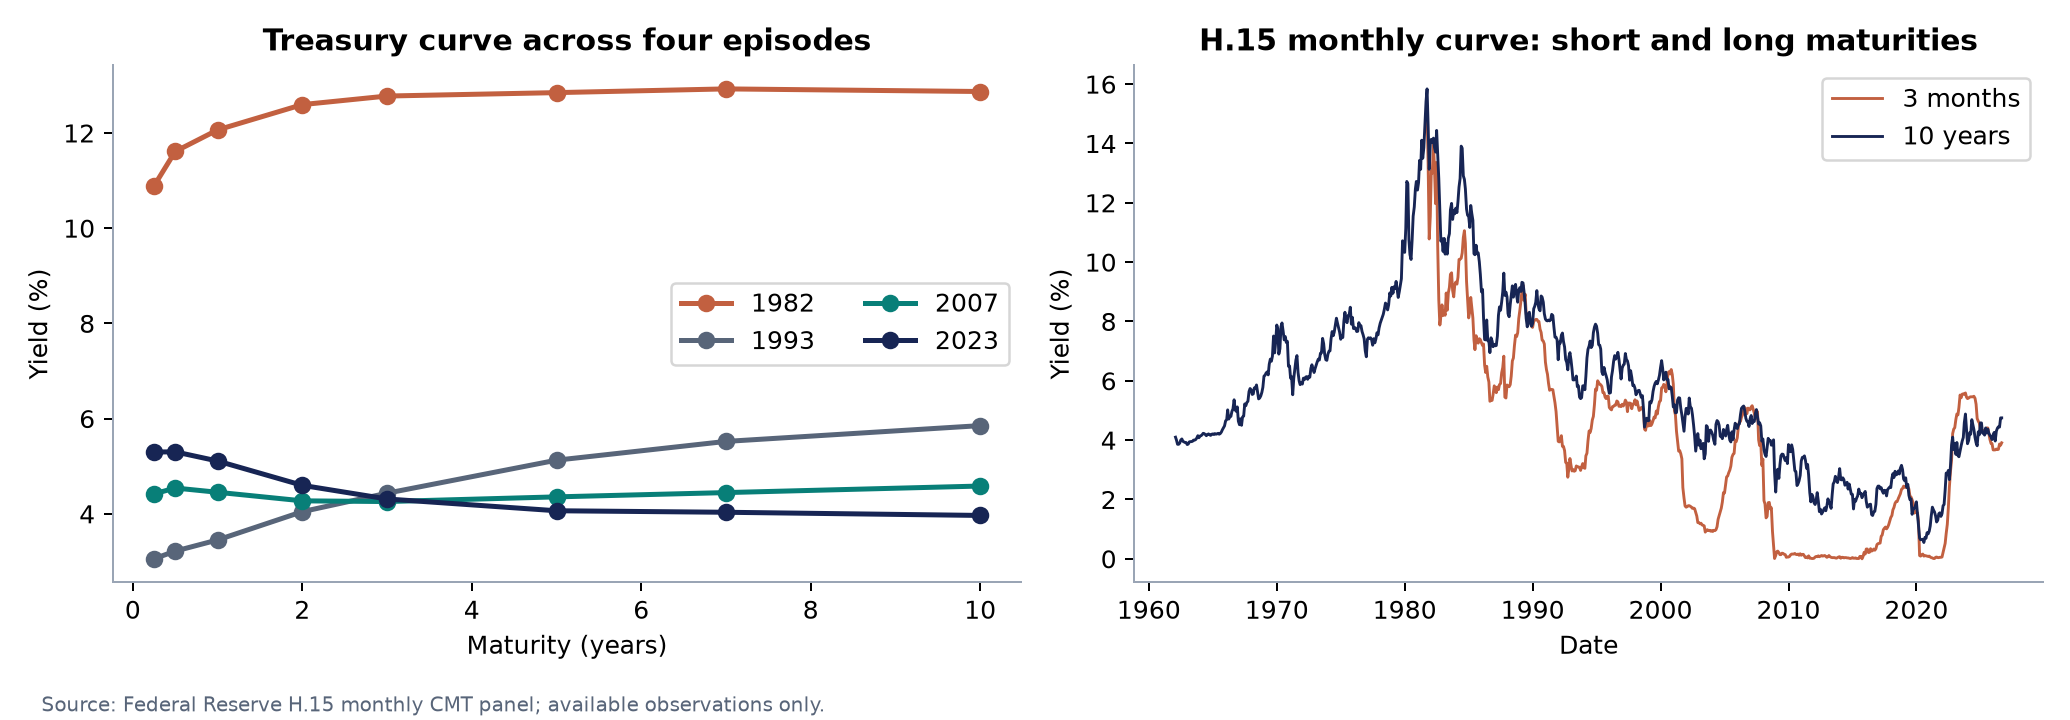
\includegraphics[width=\linewidth]{../figures/01_treasury_yields.png}
\caption{The public H.15 Treasury CMT panel. Annual average curves appear on the left and short and long maturities over time on the right. These par yields differ from the CRSP zero-coupon panel used for JKV calibration.}\label{fig.yields}
\end{figure}

We use two monthly panels and keep them separate throughout, because they differ in yield concept, maturity grid and construction.

\paragraph{Fama--Bliss (JKV).} The CRSP unsmoothed Fama--Bliss zero-coupon yields \citep{FamaBliss1987} supplied with \citet{JKV2014} through the \emph{Journal of Applied Econometrics} data archive: January 1970 to December 2009, $T=480$, and 17 maturities (3, 6, 9, 12, 15, 18, 21, 24, 30, 36, 48, 60, 72, 84, 96, 108 and 120 months) with no missing values. The yields are bootstrapped from bond prices without fitting a curve.

\paragraph{Treasury CMT.} The official Treasury constant-maturity par yields, month-end, from the Federal Reserve's H.15 release (identical to the treasury.gov par curve from 1990): September 1981 to August 2026, $T=540$. Only eight maturities---3 and 6 months and 1, 2, 3, 5, 7 and 10 years---are available without gaps over the whole span; the 1-month (from 2001), 2- and 4-month (from 2018), 20-year (missing 1987--93) and 30-year (missing 2002--06) series are dropped rather than interpolated, so $N=8$. We also report a shorter panel, 1990--2026 ($T=440$), restricted to treasury.gov data. Treasury changed its curve-fitting method in December 2021, 57 months before the end of the sample; we have not tested separately whether this change contributes to the rejections, but the 1981--2026 and 1990--2026 results are close to those of samples ending in 2009 (Table~\ref{tab.sub}).

\paragraph{GSW.} The fitted Svensson curve of \citet{GSW2007} is used only for comparison. Because it is itself the output of a fitted Nelson--Siegel/Svensson model, it is not used for testing.

The two panels differ: zero-coupon versus par yields, 17 versus 8 maturities, and 1970--2009 versus 1981--2026. We compare results side by side and never pool them. The small $N$ of the Treasury panel costs power, which the simulations in Section~\ref{sec.mc} quantify. 

\section{Monte Carlo evidence at our sample sizes}\label{sec.mc}

SW's simulations use $N,T\in\{100,200\}$. Our panels have $N=8$ or 17 and $T$ near 500, so we check size and power at these dimensions before turning to the data.

\subsection{SW's designs}

We first run SW's DGPs 1--7 \citep[Section 5.3]{SuWang2017} with two true factors at $N\in\{8,11,15,17,20\}$ and $T\in\{100,200\}$, plus the two empirical dimensions, with 500 replications. These runs use $B=199$ and add-one $p$-values rather than SW's $B=200$ and $p^*$. DGPs 1--3 impose constant loadings with i.i.d., heteroskedastic and cross-correlated errors; DGPs 4--7 let the loadings change through a single break, multiple breaks, or smooth drift, with magnitude $b\in\{1,2\}$.

Table~\ref{tab.swsize} reports the size at the 5\% level. On the grid the largest rejection rate is 5.4\% (1.4\% at the 1\% level), and most cells are below nominal. At the Fama--Bliss dimensions ($N=17$, $T=480$) size is 3.4\%, 7.4\% and 5.2\% under DGPs 1--3. The 7.4\% under heteroskedastic errors is about 2.4 Monte Carlo standard errors above 5\%, a mild over-rejection; it is far too small to matter for the empirical rejections, whose $p$-values are mostly at the floor of 0.0001. As a benchmark, at $N=T=100$ under DGP 1 the size of our implementation is 0.6\% in this grid (and 1.2\% in the separate 300-replication comparison of Appendix~\ref{app.bootstrap}), against 6.4\% in SW's Table 3; the difference is explained by the bootstrap in SW's released code.

\begin{table}[htbp]
\centering
\begin{threeparttable}
\caption{Size of the test under SW's DGPs at small $N$ (rejection rate, \%, 5\% level)}\label{tab.swsize}
\begin{tabular}{lccccc}
\toprule
DGP, $T$ & $N=8$ & $N=11$ & $N=15$ & $N=17$ & $N=20$\\
\midrule
1 i.i.d., 100 & 3.0 & 0.0 & 1.0 & 1.8 & 2.2\\
1 i.i.d., 200 & 2.4 & 1.4 & 3.2 & 3.4 & 3.4\\
2 heterosk., 100 & 3.8 & 3.6 & 0.6 & 1.6 & 0.6\\
2 heterosk., 200 & 2.4 & 4.2 & 2.6 & 5.2 & 3.2\\
3 cross-corr., 100 & 3.6 & 3.0 & 2.2 & 2.2 & 3.4\\
3 cross-corr., 200 & 3.6 & 1.8 & 4.0 & 2.6 & 5.4\\
\midrule
\multicolumn{6}{l}{At the Fama--Bliss dimensions ($N=17$, $T=480$): DGP 1: 3.4; DGP 2: 7.4; DGP 3: 5.2}\\
\bottomrule
\end{tabular}
\begin{tablenotes}\small
\item Notes: 500 replications, $B=199$, two true factors, printed (covariance) bootstrap. The Monte Carlo standard error at 5\% is about 1.0 point.
\end{tablenotes}
\end{threeparttable}
\end{table}

Table~\ref{tab.swpower} reports power. At the Fama--Bliss dimensions every design rejects in at least 91.8\% of replications when $b=1$. At the Treasury dimensions ($N=8$, $T=540$) power is high against breaks (96.6--100\%) and against DGP 7, but only 31.8\% against the slow drift of DGP 6 with $b=1$. With $N=8$ and $T=200$ the test has essentially no power against that drift (3.0\%, below the nominal level). A failure to reject in the Treasury panel would therefore carry little weight against slow drift; as it happens, the Treasury panel rejects at every rank.

\begin{table}[htbp]
\centering
\begin{threeparttable}
\caption{Power of the test under SW's DGPs (rejection rate, \%, 5\% level)}\label{tab.swpower}
\begin{tabular}{lccccccc}
\toprule
 & \multicolumn{5}{c}{$T=200$} & \multicolumn{2}{c}{Empirical dimensions}\\
\cmidrule(lr){2-6}\cmidrule(lr){7-8}
DGP, $b$ & $N=8$ & 11 & 15 & 17 & 20 & $17\times480$ & $8\times540$\\
\midrule
4 break, 1 & 95.8 & 79.6 & 100.0 & 99.8 & 100.0 & 100.0 & 100.0\\
4 break, 2 & 93.0 & 85.8 & 98.4 & 100.0 & 100.0 & & \\
5 breaks, 1 & 59.4 & 28.4 & 89.6 & 98.2 & 100.0 & 99.8 & 96.6\\
5 breaks, 2 & 97.8 & 94.0 & 99.4 & 99.8 & 100.0 & & \\
6 smooth, 1 & 3.0 & 23.4 & 51.4 & 47.4 & 50.6 & 91.8 & 31.8\\
6 smooth, 2 & 91.2 & 90.8 & 99.4 & 100.0 & 100.0 & & \\
7 smooth, 1 & 72.0 & 86.8 & 52.2 & 99.2 & 100.0 & 100.0 & 94.6\\
7 smooth, 2 & 84.2 & 75.0 & 90.6 & 99.8 & 83.6 & & \\
\bottomrule
\end{tabular}
\begin{tablenotes}\small
\item Notes: 500 replications, $B=199$. Loadings are drawn once per cell, as in SW, which explains the non-monotone pattern across $N$; at $T=100$ (not shown) power depends strongly on that draw (for DGP 4, $b=1$, five draws give 19--89\% at $N=11$), while size is unaffected.
\end{tablenotes}
\end{threeparttable}
\end{table}

\subsection{Fake yield curves calibrated to each panel}

SW's DGPs are generic. To check the test on data that look like yield curves, we generate fake panels from Nelson--Siegel (three-factor) and Svensson (four-factor) loadings fitted to each real panel, with a shared first decay parameter so that the three-factor model nests in the four-factor one ($\kappa_1=0.0636$, $\kappa_2=0.0359$ for the Fama--Bliss maturities). Factors follow AR(1) processes estimated from the real data, and each maturity receives i.i.d.\ $N(0,s_i^2)$ noise, with $s_i$ the standard deviation of the real residual of that maturity (5--14 basis points with three factors). Three setups are considered: three factors throughout (\emph{null3}); four throughout (\emph{null4}); and three factors for 240 months followed by four (\emph{break}). In the \emph{break} setup the Svensson loadings are the same throughout and the fourth factor is zero in the first half, so the change is in the factor structure rather than in the loadings of the factors already present. All fake panels have $T=480$, so that the two calibrations share one design and coincide with the scan simulations of Section~\ref{sec.scan}; with the Treasury grid ($N=8$) this gives $Th=76.9$ months rather than the 84.5 of the real Treasury panel. Following SW, we use 500 data sets, $B=200$ and $p^*$.

\begin{table}[htbp]
\centering
\begin{threeparttable}
\caption{Size and power on calibrated Nelson--Siegel/Svensson fake curves (rejection rate, \%)}\label{tab.fakesize}
\begin{tabular}{lllcccccc}
\toprule
 & & & \multicolumn{3}{c}{JKV-calibrated} & \multicolumn{3}{c}{Treasury-calibrated}\\
\cmidrule(lr){4-6}\cmidrule(lr){7-9}
 & True structure & $d$ & 1\% & 5\% & 10\% & 1\% & 5\% & 10\%\\
\midrule
Size & 3 factors & 3 & 0.2 & 2.0 & 4.4 & 0.8 & 3.6 & 6.4\\
Size & 4 factors & 4 & 0.4 & 3.4 & 7.2 & 1.0 & 4.2 & 8.4\\
Size, $d$ too large & 3 factors & 4 & 0.6 & 2.6 & 8.0 & 0.6 & 2.6 & 8.4\\[3pt]
Power & 4 factors & 3 & 97.4 & 99.2 & 99.4 & 99.2 & 100.0 & 100.0\\
Power & $3\to4$ at month 240 & 3 & 99.8 & 100.0 & 100.0 & 97.8 & 99.4 & 99.4\\
Factor appears & $3\to4$ at month 240 & 4 & 93.6 & 99.6 & 99.8 & 95.2 & 99.2 & 99.6\\
\bottomrule
\end{tabular}
\begin{tablenotes}\small
\item Notes: $T=480$, 500 data sets, $B=200$, $p^*$ as in SW; rule-of-thumb bandwidth ($Th=71.4$ months on the JKV grid, 76.9 on the Treasury grid). Monte Carlo standard errors at the nominal level are 0.4, 1.0 and 1.3 points at 1\%, 5\% and 10\%. In the last row the Svensson loadings are constant and the fourth factor is zero before month 240.
\end{tablenotes}
\end{threeparttable}
\end{table}

Table~\ref{tab.fakesize} shows no sign of over-rejection at any level in either calibration: no size entry exceeds its nominal level by more than two Monte Carlo standard errors, and the three-factor JKV design is clearly conservative (2.0\% at 5\%). The same holds when the test is run with one factor too many (row ``$d$ too large''), which supports the use of Proposition~\ref{prop.rank}. Power is at least 97\% at the 1\% level, both against a fourth factor present throughout and against a change from three to four factors in mid-sample. The last row illustrates the equivalence noted in Section~\ref{sec.test}: when a fourth factor appears in mid-sample, the test at $d=4$ rejects in 94--96\% of runs at 1\%, although the Svensson loadings never change. In SW's normalization this is a loading change.

The calibrated noise is independent over time, which is what both the bootstrap and SW's theory assume. The residuals of the constant-loading fits to the real panels have lag-one autocorrelations of 0.5--0.7, so these experiments establish that the test is correctly sized under its own assumptions, not that the empirical rejections are robust to serial correlation in the errors. Section~\ref{sec.ar} relaxes this assumption.

\subsection{A benchmark for size, power and dating}\label{sec.bench}
\begin{figure}[htbp]
\centering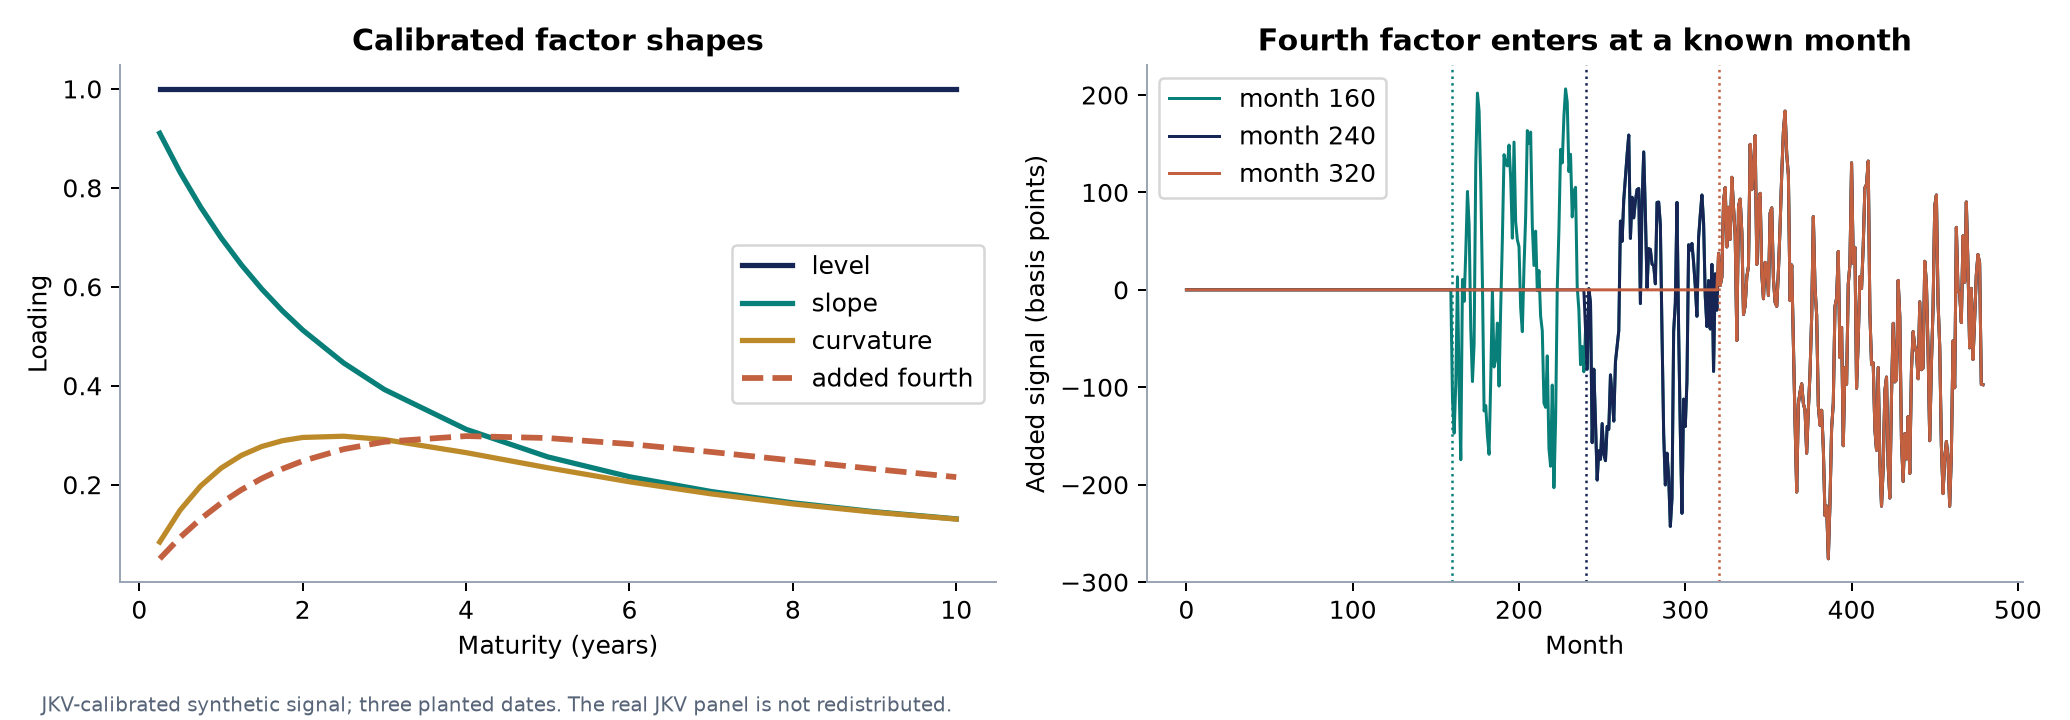
\includegraphics[width=\linewidth]{../figures/02_simulation_design.png}
\caption{Calibrated loadings and the planted fourth-factor signal. The original three factors continue throughout; only the fourth switches on at the known month. This alternative differs from the fixed-rank changing-loading designs in \citet{SuWang2017}.}\label{fig.design}
\end{figure}

\begin{figure}[htbp]
\centering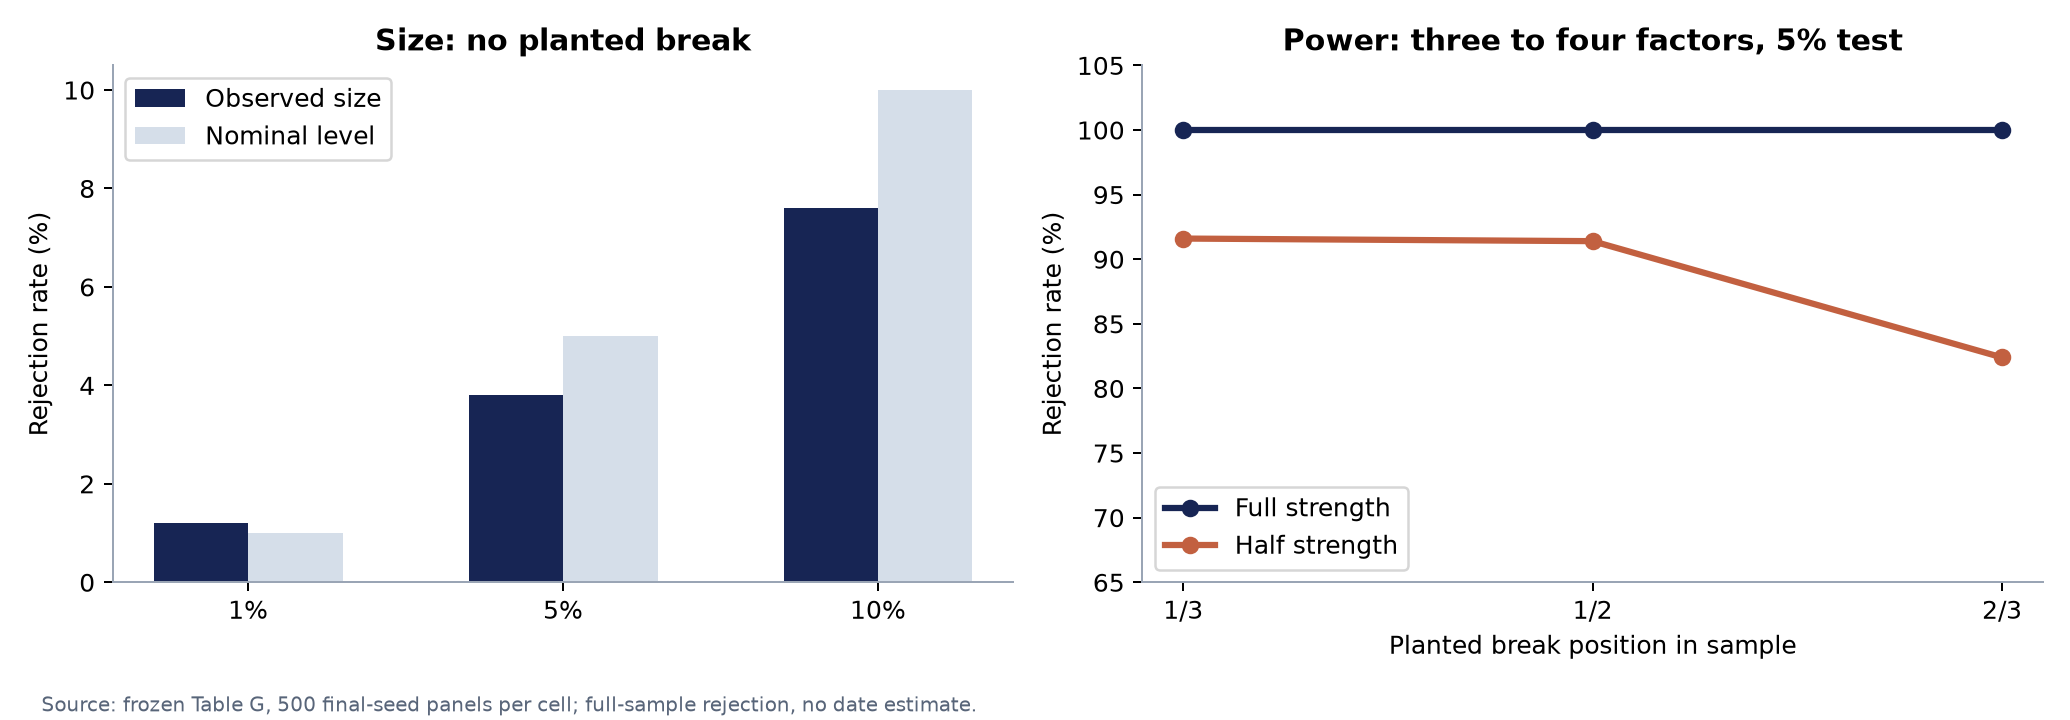
\includegraphics[width=\linewidth]{../figures/03_fullsample_size_power.png}
\caption{Full-sample rejection frequencies from 500 final-seed panels per cell. Size uses no-break panels; power uses a fourth factor planted at three positions. Neither outcome measures dating accuracy.}\label{fig.sizepower}
\end{figure}

The experiments above use one break position and change the factor variances and the noise together with the factor structure. For a cleaner benchmark (our week-9 design) we fix the following and use it for every procedure in this section and in Section~\ref{sec.scan}. Fake panels are calibrated to the Fama--Bliss panel ($T=480$, $N=17$) and tested at $d=3$. The three Nelson--Siegel factors follow one continuous AR(1) path through the whole sample, and the noise is i.i.d.\ over time with the standard deviation of the three-factor residual of each maturity. Under the null (\emph{null3}) the panel has three factors throughout. Under the alternative (\emph{break}) a fourth (Svensson) factor, multiplied by a strength $s$, enters at $\tau\in\{160,240,320\}$, one third, one half and two thirds of the sample; nothing else changes at $\tau$. With $s=1$ the fourth factor has its fitted size; its loading lies 95\% in the span of the first three loadings, so it is a weak factor, and we also report $s=0.5$. \emph{Size} is the share of null panels on which a procedure reports any break (or rejects); \emph{power} is the share of break panels with a break reported at or after $\tau-12$; the dating error is the first reported break minus $\tau$. Seeds are split into a tuning block, used to choose among procedures, and a final block used once. The test uses SW's $B=200$.

\begin{table}[htbp]
\centering
\begin{threeparttable}
\caption{Full-sample test on the benchmark (rejection rate, \%)}\label{tab.bench}
\begin{tabular}{lccc}
\toprule
 & 1\% & 5\% & 10\%\\
\midrule
Size, tuning seeds & 0.4 & 2.0 & 5.0\\
Size, final seeds & 1.2 & 3.8 & 7.6\\
Power, $s=1$, $\tau=160/240/320$ & 99.8 / 99.6 / 100 & 100 / 100 / 100 & 100 / 100 / 100\\
Power, $s=0.5$, $\tau=160/240/320$ & 76.5 / 77.0 / 66.0 & 89.5 / 87.5 / 78.5 & 92.0 / 92.0 / 84.0\\
\bottomrule
\end{tabular}
\begin{tablenotes}\small
\item Notes: 500 null panels per seed block; power from 500 (strength 1) and 200 (strength 0.5) tuning panels. Monte Carlo standard errors of the final-seed size are 0.5, 0.9 and 1.2 points.
\end{tablenotes}
\end{threeparttable}
\end{table}

Table~\ref{tab.bench} confirms that with independent errors the test is correctly sized (slightly conservative) and powerful; power falls when the change is weaker or later, because fewer months follow it. Table~\ref{tab.benchbw} scales the bandwidth by $c$. A narrower bandwidth raises both size and power, and the rule of thumb ($c=1$) is valid and slightly conservative; at $c=0.5$ the size at 10\% is 11.0\%. The gain from narrowing is small, so we keep SW's rule.

\begin{table}[htbp]
\centering
\begin{threeparttable}
\caption{Full-sample test: bandwidth $h=c\times$ rule of thumb (\%, 300 tuning panels, $\tau=240$)}\label{tab.benchbw}
\begin{tabular}{lcccccc}
\toprule
 & \multicolumn{3}{c}{Size} & \multicolumn{3}{c}{Power, $s=0.5$}\\
\cmidrule(lr){2-4}\cmidrule(lr){5-7}
$c$ & 1\% & 5\% & 10\% & 1\% & 5\% & 10\%\\
\midrule
0.5 & 0.3 & 4.3 & 11.0 & 81.7 & 93.0 & 96.0\\
0.75 & 0.7 & 2.7 & 7.7 & 78.3 & 91.0 & 94.3\\
1 & 0.7 & 2.3 & 5.0 & 75.0 & 87.3 & 91.7\\
1.5 & 0.7 & 1.7 & 4.0 & 71.0 & 83.0 & 89.0\\
2 & 0.7 & 2.0 & 4.0 & 69.3 & 81.3 & 86.7\\
\bottomrule
\end{tabular}
\end{threeparttable}
\end{table}

\begin{figure}[htbp]
\centering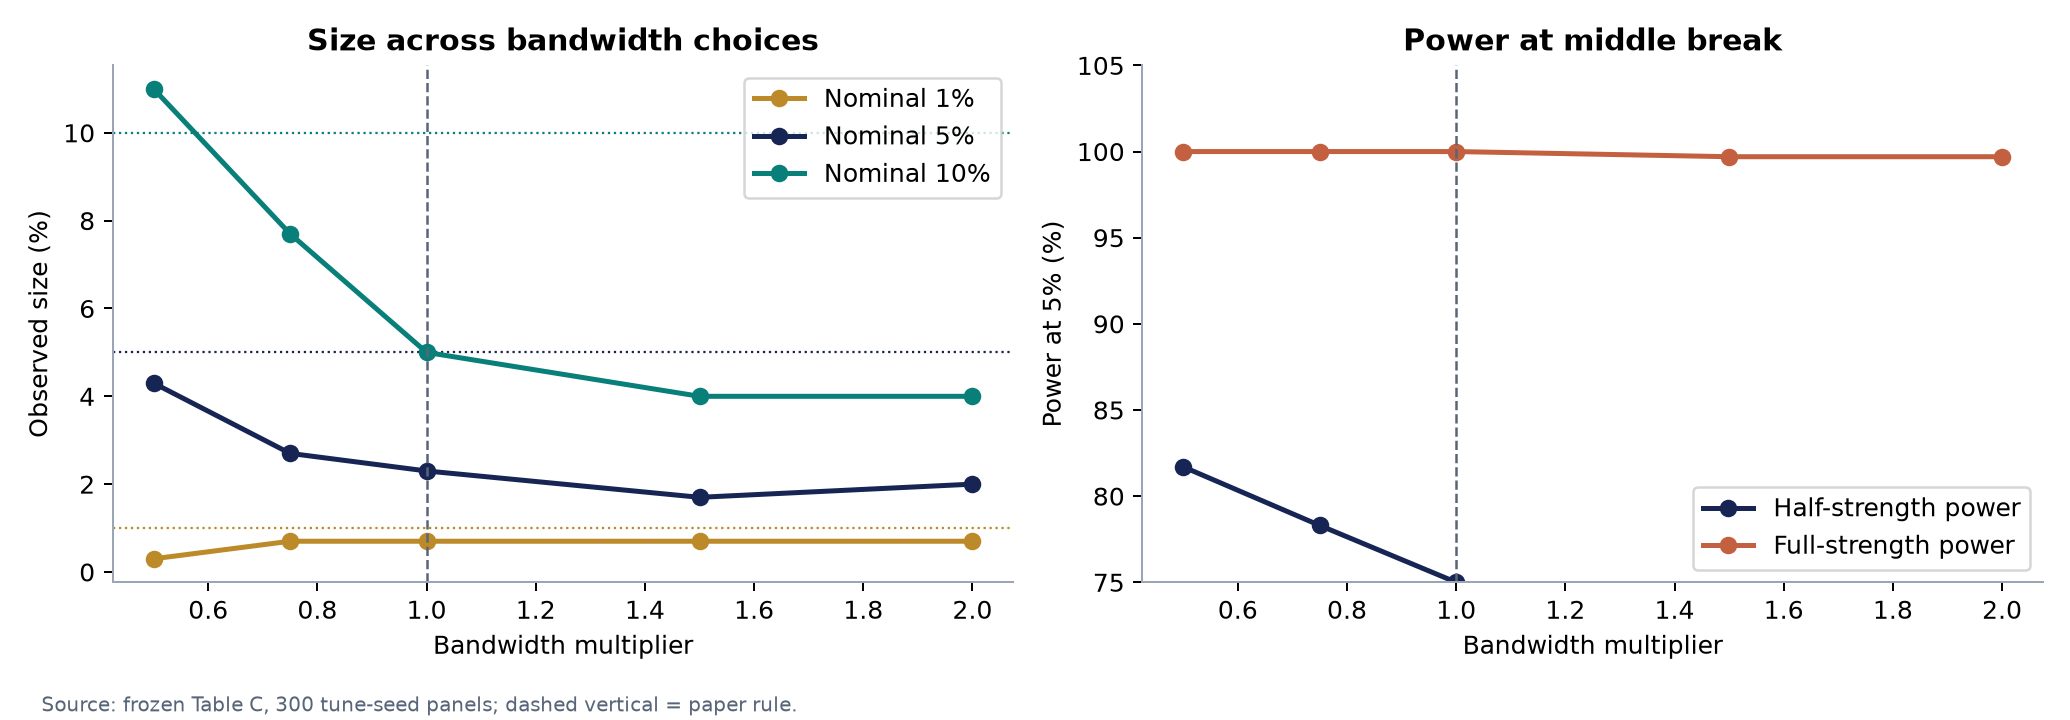
\includegraphics[width=\linewidth]{../figures/04_bandwidth.png}
\caption{Bandwidth sensitivity of full-sample size and power. The dashed vertical line is the paper's rule ($c=1$); horizontal dotted lines are nominal size levels. Results use 300 tuning panels and a middle-sample break.}\label{fig.bandwidth}
\end{figure}

\subsection{Serially correlated errors}\label{sec.ar}
\begin{figure}[htbp]
\centering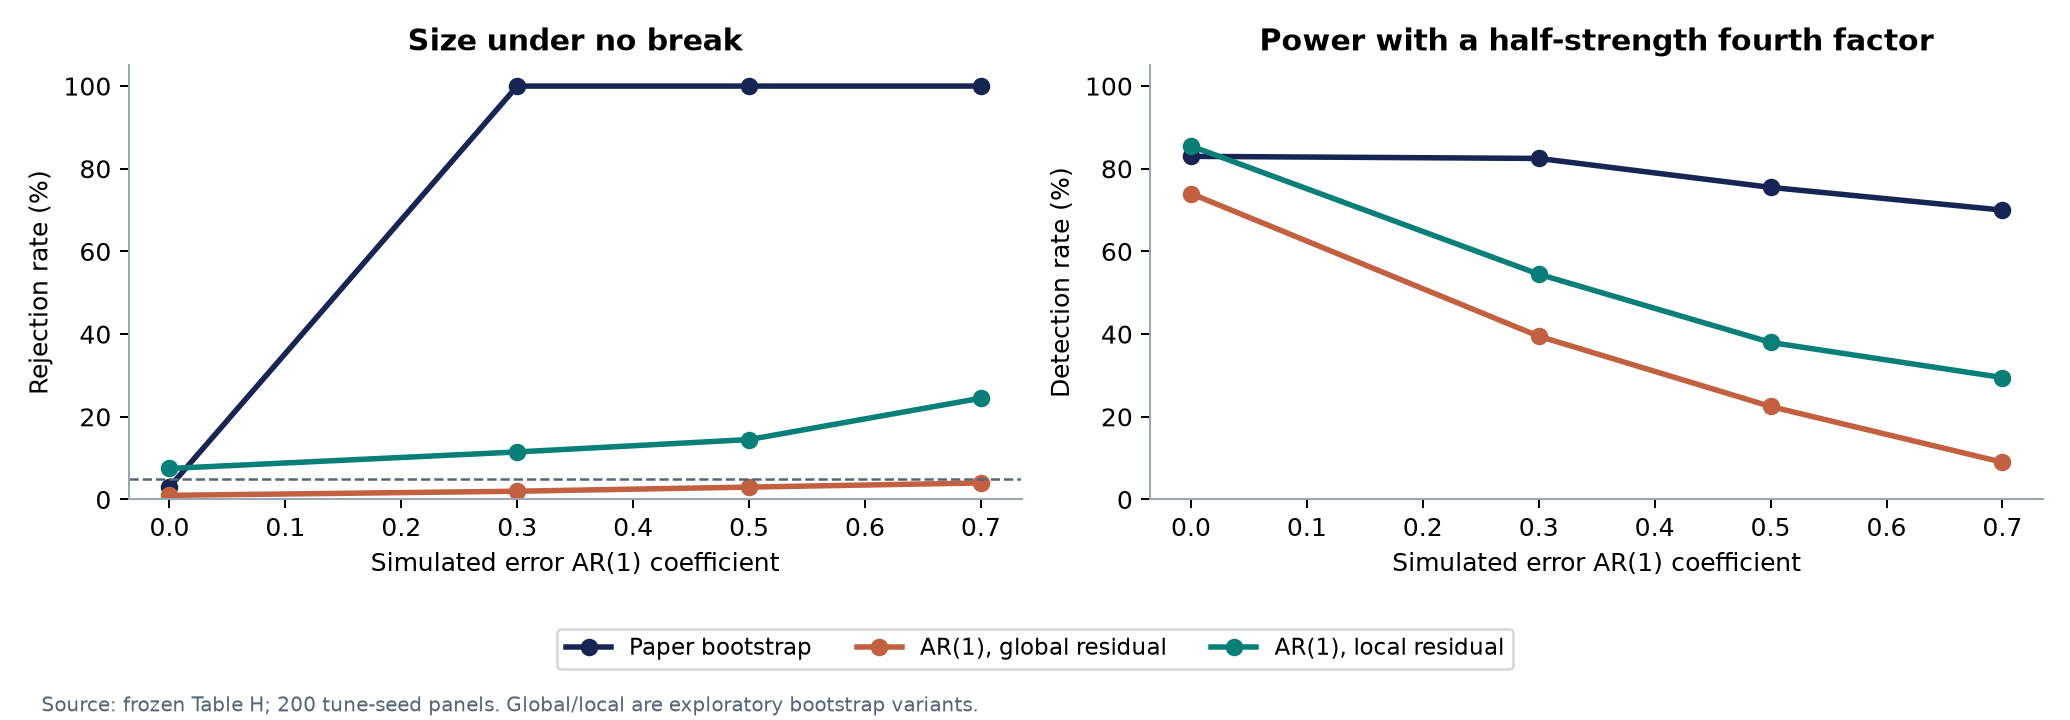
\includegraphics[width=\linewidth]{../figures/05_serial_dependence.png}
\caption{Serial-correlation stress test based on Table~\ref{tab.ar}. Size uses no-break panels; power uses a half-strength fourth factor. The global- and local-residual AR(1) bootstraps are experimental variants, not adopted corrections.}\label{fig.ar}
\end{figure}

Removing three principal components from the Fama--Bliss panel leaves residuals with a median lag-one autocorrelation of 0.63 (0.36--0.79 across maturities). We therefore replace the i.i.d.\ noise of the benchmark by AR(1) noise with coefficient $\rho$, keeping its marginal variance. Table~\ref{tab.ar} reports the full-sample test at 5\% (the gate of the ``test, then split'' procedure of Section~\ref{sec.scan}, so its size is the test's size). With SW's bootstrap the size is 3\% at $\rho=0$ and 100\% at $\rho\ge 0.3$. Persistent noise inflates the gap between the local and the global fit by roughly $(1+\rho)/(1-\rho)$; at $\rho=0.5$ the statistic rises from 0.5--1 to 8--9, against a 5\% critical value of about 2. The sequential scan of Section~\ref{sec.scan} is affected in the same way: at $\rho=0.5$ it reports a break in every null panel, 3.7 on average.

As \emph{our addition} we tried an AR(1)-sieve version of the bootstrap that draws AR(1) noise with each maturity's estimated coefficient. When the coefficient is estimated from the residual of the constant-loading fit, the size is controlled (1--4\%) but power collapses as $\rho$ grows, partly because under the alternative that residual contains the omitted fourth factor and its autocorrelation is overstated. When it is estimated from the residual of the local fit, power recovers but the size is 7.5--24.5\%, because the local fit absorbs part of the noise. Neither version is satisfactory. Section~\ref{sec.robust} returns to this problem and changes the statistic as well as the bootstrap.

\begin{table}[htbp]
\centering
\begin{threeparttable}
\caption{Full-sample test at 5\% with AR(1) errors (\%, 200 tuning panels, $\tau=240$)}\label{tab.ar}
\begin{tabular}{lcccc}
\toprule
Bootstrap, $\rho$ & 0 & 0.3 & 0.5 & 0.7\\
\midrule
\multicolumn{5}{l}{\emph{Size}}\\
SW (i.i.d.\ over time) & 3.0 & 100 & 100 & 100\\
AR(1), constant-loading residual & 1.0 & 2.0 & 3.0 & 4.0\\
AR(1), local residual & 7.5 & 11.5 & 14.5 & 24.5\\[3pt]
\multicolumn{5}{l}{\emph{Power, strength 0.5}}\\
SW (i.i.d.\ over time) & 83.0 & 82.5 & 75.5 & 70.0\\
AR(1), constant-loading residual & 74.0 & 39.5 & 22.5 & 9.0\\
AR(1), local residual & 85.5 & 54.5 & 38.0 & 29.5\\
\bottomrule
\end{tabular}
\begin{tablenotes}\small
\item Notes: rates of the ``test, then split'' procedure of Section~\ref{sec.scan} at 5\%; power counts a break dated at or after $\tau-12$. Power under SW's bootstrap with $\rho>0$ is not meaningful because its size is 100\%.
\end{tablenotes}
\end{threeparttable}
\end{table}

\section{Empirical results}\label{sec.results}

\subsection{Full sample}

Table~\ref{tab.full} reports the full-sample tests. In the Treasury panel constant loadings are rejected at $d=3$, 4 and 5, both over 1981--2026 and over 1990--2026. The observed statistic exceeds its bootstrap 99\% critical value many times over at $d=3$ and $d=4$, and by a smaller margin at $d=5$ ($p=0.0012$). In the Fama--Bliss panel the test rejects at $d=3$ ($\hat J_{NT}=91.0$ against a 99\% critical value of 24.7) but not at $d=4$ ($p=0.342$) or $d=5$ ($p=0.247$).

\begin{table}[htbp]
\centering
\begin{threeparttable}
\small
\caption{Full-sample tests of constant loadings}\label{tab.full}
\begin{tabular}{lcccc}
\toprule
Panel & & $d=3$ & $d=4$ & $d=5$\\
\midrule
\multirow{2}{*}{JKV 1970--2009 ($N=17$, $T=480$)} & $\hat J_{NT}$ / crit.\ 99\% & 91.0 / 24.7 & 65.1 / 86.8 & 79.3 / 92.1\\
 & $p$ & $\le 0.0001$ & 0.342 & 0.247\\[3pt]
\multirow{2}{*}{Treasury 1981--2026 ($N=8$, $T=540$)} & $\hat J_{NT}$ / crit.\ 99\% & 108.8 / 6.9 & 92.2 / 19.9 & 117.1 / 99.8\\
 & $p$ & $\le 0.0001$ & $\le 0.0001$ & 0.0012\\[3pt]
\multirow{2}{*}{Treasury 1990--2026 ($N=8$, $T=440$)} & $\hat J_{NT}$ / crit.\ 99\% & 115.6 / 5.6 & 95.0 / 19.8 & 93.2 / 82.7\\
 & $p$ & $\le 0.0001$ & $\le 0.0001$ & 0.0012\\
\bottomrule
\end{tabular}
\begin{tablenotes}\small
\item Notes: rule-of-thumb bandwidth (\ref{eq.bandwidth}) for each panel; printed bootstrap with $B=9{,}999$; add-one $p$-values (smallest attainable 0.0001). An independent re-run of the Treasury 1981--2026, $d=5$ test with a different seed gives $p=0.0005$; every other decision is likewise unchanged across runs. 
\end{tablenotes}
\end{threeparttable}
\end{table}

By Proposition~\ref{prop.rank}, the Treasury rejections at $d=5$ are evidence against every constant-loading model with five or fewer factors for the official Treasury curve since 1981, including Nelson--Siegel and Svensson, subject to the qualifications in Section~\ref{sec.discussion}. The Fama--Bliss rejection at $d=3$ is evidence against constant three-factor models, including the dynamic Nelson--Siegel model, over 1970--2009.

\subsection{Why the Fama--Bliss panel does not reject at $d=4$}

The non-rejection at $d=4$ in the Fama--Bliss panel is associated with the early 1970s. As a sensitivity analysis---not a pre-specified test---we re-ran the full test with the end date fixed at December 2009 and the start year moved from 1970 to 1986 (17 tests). The test rejects at $d=4$ for every start between 1977 and 1986 and does not reject for starts in 1970--1976. The months 1970--76 make up 18\% of the sample but 30\% of the residual sum of squares of the constant four-factor fit; the high-inflation and disinflation years 1977--82 make up a further 15\% of the months and 32\% of the misfit.

This misfit enters the test in two ways. It raises $\hat J_{NT}$, but it also enters the restricted residuals from which the bootstrap samples are built, which raises the bootstrap null distribution. Moving the start from 1980 to 1970 raises the median bootstrap $\hat J^*_{NT}$ from 21 to 61, while the observed $\hat J_{NT}$ rises only from 40 to 65; the 99\% critical value rises from 37 to 87, and the test no longer rejects. This pattern is consistent with a loss of power caused by the turbulent 1970s, rather than with evidence in favour of constant loadings. Heteroskedasticity or serial correlation concentrated in the 1970s could produce the same pattern, and the exercise does not distinguish among these.

\subsection{Bandwidth}

The bandwidth decides how many months the local fit pools. With $Th=71$ months, a change that lasts a few years is averaged with the years around it and the local fit is close to the global one. Table~\ref{tab.bw} reports the Fama--Bliss tests at fixed narrower bandwidths. At $d=3$ every bandwidth rejects; at $d=4$ the $p$-value falls from 0.342 at the rule-of-thumb bandwidth to 0.0115 at $Th=36$ and to at most 0.0001 at $Th\le 24$. In the Treasury panel every combination rejects at 1\%. In a separate set of runs with the rule-of-thumb bandwidth scaled by 0.5, 0.8, 1, 1.2 and 2 (each with its own bootstrap), the Fama--Bliss panel rejects at $d=3$ for all five bandwidths, at $d=4$ only at $0.5\times$ ($Th=36$ months, $p=0.0095$, a different bootstrap run from the $p=0.0115$ in Table~\ref{tab.bw}), and at $d=5$ for none; the Treasury panel rejects at every $d$ and every bandwidth. The $d=4$ decision at $Th\approx36$ months is therefore borderline at 1\%.

\begin{table}[htbp]
\centering
\begin{threeparttable}
\caption{Full-sample $p$-values of the JKV panel at narrower bandwidths}\label{tab.bw}
\begin{tabular}{lcccc}
\toprule
$Th$ (months) & 71.4 (rule of thumb) & 36 & 24 & 12\\
\midrule
$d=3$ & $\le 0.0001$ & $\le 0.0001$ & $\le 0.0001$ & $\le 0.0001$\\
$d=4$ & 0.342 & 0.0115 & $\le 0.0001$ & $\le 0.0001$\\
$d=5$ & 0.247 & 0.212 & 0.0017 & 0.0425\\
\bottomrule
\end{tabular}
\begin{tablenotes}\small
\item Notes: JKV 1970--2009; $B=9{,}999$; only $h$ changes along a row. The size of the test at bandwidths narrower than the rule of thumb has not been studied separately.
\end{tablenotes}
\end{threeparttable}
\end{table}

\subsection{Sub-samples and the two panels compared}

Table~\ref{tab.sub} repeats the test on sub-samples, each with its own standardization, bandwidth and bootstrap. The test rejects at $d=3$ in all eight samples and at $d=4$ in six. Over the common window 1990--2009 the two panels give the same decision at every rank: reject at $d=3$ and $d=4$, do not reject at $d=5$. The post-crisis Treasury sample 2010--2026 rejects only at $d=3$.

\begin{table}[htbp]
\centering
\begin{threeparttable}
\caption{Sub-samples: ratio of $\hat J_{NT}$ to its bootstrap 99\% critical value}\label{tab.sub}
\begin{tabular}{lcccccccc}
\toprule
 & \multicolumn{4}{c}{JKV zero-coupon} & \multicolumn{4}{c}{Treasury par}\\
\cmidrule(lr){2-5}\cmidrule(lr){6-9}
 & 1970--09 & 1977--09 & 1983--09 & 1990--09 & 1990--09 & 1990--26 & 1981--26 & 2010--26\\
$T$ & 480 & 396 & 324 & 240 & 240 & 440 & 540 & 200\\
\midrule
$d=3$ & \textbf{3.73} & \textbf{6.85} & \textbf{9.06} & \textbf{3.88} & \textbf{6.43} & \textbf{21.53} & \textbf{15.69} & \textbf{6.96}\\
$d=4$ & 0.73 & \textbf{1.10} & \textbf{3.17} & \textbf{1.20} & \textbf{2.66} & \textbf{4.69} & \textbf{4.47} & 0.94\\
$d=5$ & 0.86 & 0.82 & \textbf{1.20} & 0.88 & 0.81 & \textbf{1.14} & \textbf{1.16} & 0.85\\
\bottomrule
\end{tabular}
\begin{tablenotes}\small
\item Notes: bold = rejection at 1\% (ratio above one). Each cell is a separate test with its own rule-of-thumb bandwidth and $B=1{,}999$.
\end{tablenotes}
\end{threeparttable}
\end{table}

\section{When do the loadings change? Two dating procedures}\label{sec.scan}

This section goes beyond SW, whose simulations evaluate rejection rates only, and is secondary to the full-sample results of Sections~\ref{sec.mc} and \ref{sec.results}. The full-sample test answers question (1) of the introduction. To date a change (question 2) a procedure must do two things: decide whether there is a change, and estimate when. A \emph{sequential scan} does both with the same tool, by applying the test to growing windows and recording the first window that rejects. This has two structural costs. Because many windows are tested, the false-alarm rate of the procedure is larger than the level of each test. And because a window rejects only after enough post-change months have accumulated, the recorded date lags the change. The alternative we consider, \emph{test, then split}, separates the two tasks: the full-sample test decides once, so the procedure inherits its size, and the date is estimated by least squares. Both are evaluated on the benchmark of Section~\ref{sec.bench}. 

\subsection{Procedure}

To locate changes we apply the test sequentially, separately for each $d$. Starting from the beginning of the sample, we test windows of 60, 61, 62, \ldots\ months. The first month whose inclusion makes the window reject at 1\% is recorded as a break (a 999-draw screen, confirmed with 9,999 draws). If the very first 60-month window already rejects, we shrink it one month at a time until it no longer rejects and record that boundary as the break (``retreat''). After a break the next segment starts at the break month and testing resumes once 60 new months are available. Each window is standardized on its own data.

This procedure follows the forward search outlined in our original research plan, with two operational choices. The plan starts from an initial sample in which $H_0$ is not rejected; the retreat step implements this when the first window already rejects, so that the recorded date is a boundary of a non-rejecting stretch rather than the edge of the first window. The 60-month minimum window and restart window are our choice; Section~\ref{sec.scanres} reports their effect.

Two bandwidth rules are considered. Under the \emph{per-window} rule, $h$ follows (\ref{eq.bandwidth}) with the window's own $T$, so the effective half-window $Th$ grows from about 14 months in a 60-month window to 71 in the full Fama--Bliss sample. Under the \emph{full-sample} rule, every window reuses the full sample's $Th$ (71.4 months for JKV, 84.5 for Treasury). In a short window this implies $h>1/2$ and the two boundary regions in (\ref{eq.boundary}) overlap; we then truncate the kernel on both sides and renormalize (Appendix~\ref{app.kernel}). Bandwidths with $h\ge 1/2$ lie outside SW's asymptotic theory, which requires $h\to 0$.

\subsection{Results}\label{sec.scanres}

Table~\ref{tab.breaks} lists the breaks under both rules. Under the per-window rule the scan finds 27 breaks across the six panel--rank combinations; at $d=4$ it finds 1981-08 and 2004-12 in the Fama--Bliss panel and 1993-06, 1999-02, 2004-03 and 2019-11 in the Treasury panel. Under the full-sample rule it finds 31. Only three of the new dates lie within three months of an old one at the same $d$, and the $d=4$ dates 1981-08 and 1993-06 move by 19 and 18 months.

\begin{table}[htbp]
\centering
\small
\begin{threeparttable}
\caption{Break dates from the sequential scan (60/60 windows, 1\% level)}\label{tab.breaks}
\begin{tabular}{llp{5.6cm}p{5.6cm}}
\toprule
Panel & $d$ & Per-window bandwidth & Full-sample bandwidth\\
\midrule
JKV & 3 & 1974-08$^\dagger$, 1977-02$^\dagger$, 1984-05, 1994-10, 1998-09$^\dagger$, 2001-07$^\dagger$, 2004-02$^\dagger$, 2006-04$^\dagger$ & 1978-03, 1982-12$^\ddagger$, 1987-06$^\ddagger$, 1992-04$^\ddagger$, 1997-06, 2001-10$^\ddagger$, 2005-10$^\ddagger$\\
JKV & 4 & 1981-08, 2004-12 & 1976-11, 1983-03, 1987-06$^\ddagger$, 1994-09, 2002-01, 2008-02\\
JKV & 5 & 1975-08, 1978-10$^\dagger$ & 1983-10, 2000-10\\[3pt]
Treasury & 3 & 1993-08, 1997-05$^\dagger$, 2001-06$^\dagger$, 2004-06$^\dagger$, 2007-10$^\dagger$, 2016-03, 2019-03$^\dagger$, 2024-08 & 1992-06, 1998-02, 2002-11$^\ddagger$, 2007-12, 2014-07, 2019-08, 2024-05$^\ddagger$\\
Treasury & 4 & 1993-06, 1999-02, 2004-03, 2019-11 & 1991-12, 1996-05$^\ddagger$, 2002-10, 2011-02, 2016-08, 2025-06\\
Treasury & 5 & 1988-11, 1994-03, 1998-08$^\dagger$ & 1986-06$^\ddagger$, 1991-07, 2022-06\\
\midrule
Total & & 27 (13 by retreat) & 31 (10 by retreat)\\
\bottomrule
\end{tabular}
\begin{tablenotes}\small
\item Notes: $^\dagger$ dated by retreat under the per-window rule (windows of 27--56 months). $^\ddagger$ dated by retreat under the full-sample rule; these windows are 49--59 months long, so the dates are set by the 60-month minimum window rather than by the data. JKV covers 1970--2009, Treasury 1981--2026.
\end{tablenotes}
\end{threeparttable}
\end{table}

Under the per-window rule the search settings also matter. Varying the first window over 24--100 months barely changes the breaks, but the restart window does: with a 24-month restart the scan finds 8 breaks at $d=4$ in the Fama--Bliss panel, against 2 with a 60-month restart. Across all restart windows (12, 24, 36 and 60 months) only two $d=4$ breaks recur within three months: JKV 1981-08 and Treasury 1993-06. Under the full-sample rule, with $Th$ fixed, a slightly shorter window barely changes the $p$-value, so the retreat dates cluster just below the 60-month minimum window (Table~\ref{tab.breaks}, $^\ddagger$). Short windows are not specific to the full-sample rule: under both rules most breaks are found in windows shorter than $2Th$ (25 of 27 and 28 of 31).

\subsection{How reliable is the scan? Earlier simulations}

We run the scan on the calibrated fake curves of Section~\ref{sec.mc} with the full-sample bandwidth, 100 runs per cell (Table~\ref{tab.scansim}). Because the scan performs many tests, its false-alarm rate is not $\alpha$. With no break, it reports at least one break in 3--14\% of runs at 1\%, 24--42\% at 5\%, and 45--60\% at 10\%; the full-sample test on the same panels rejects in 0--8\%, never above its nominal level. Under the per-window rule the JKV-calibrated false-alarm rates at 1\% are 5\% and 4\%, close to those under the full-sample rule.

When a three-to-four-factor change is planted at month 240, the scan at $d=3$ dates a break at or after month 228 in every run, but late: within three years of the change in 57--65\% of runs at 1\%, with a median delay of 27--32 months. Detection at $d=4$ is much weaker: at 1\% the scan dates a break within three years in only 20\% (JKV) and 2\% (Treasury) of runs, with median delays of 78 and 93 months. At $d=4$ the scan also reacts to the drop in residual variance that accompanies the change. Since the interpretation of dates below relies mostly on $d=4$ breaks, these numbers are an important caveat.

\begin{table}[htbp]
\centering
\begin{threeparttable}
\small
\caption{The scan on calibrated fake curves (full-sample bandwidth)}\label{tab.scansim}
\begin{tabular}{llccccc}
\toprule
\multicolumn{7}{l}{\emph{Panel A: no break}}\\
 & & \multicolumn{2}{c}{Scan: any break dated} & \multicolumn{3}{c}{Full test rejects}\\
\cmidrule(lr){3-4}\cmidrule(lr){5-7}
Calibration & $\alpha$ & 3 fac., $d=3$ & 4 fac., $d=4$ & 3 fac., $d=3$ & & \\
\midrule
JKV & 1\% & 7 & 3 & 0 & & \\
JKV & 5\% & 26 & 24 & 4 & & \\
JKV & 10\% & 47 & 45 & 5 & & \\
Treasury & 1\% & 7 & 14 & 0 & & \\
Treasury & 5\% & 28 & 42 & 5 & & \\
Treasury & 10\% & 48 & 60 & 8 & & \\
\midrule
\multicolumn{7}{l}{\emph{Panel B: three factors, then four from month 240}}\\
 & & \multicolumn{2}{c}{$d=3$} & \multicolumn{2}{c}{$d=4$} & \\
\cmidrule(lr){3-4}\cmidrule(lr){5-6}
Calibration & $\alpha$ & within 3 yrs & median delay & within 3 yrs & median delay & \\
\midrule
JKV & 1\% & 65 & 27 & 20 & 78 & \\
JKV & 5\% & 76 & 19 & 41 & 41 & \\
JKV & 10\% & 78 & 16 & 52 & 35 & \\
Treasury & 1\% & 57 & 32 & 2 & 93 & \\
Treasury & 5\% & 67 & 23 & 28 & 53 & \\
Treasury & 10\% & 66 & 23 & 50 & 35 & \\
\bottomrule
\end{tabular}
\begin{tablenotes}\small
\item Notes: rates in \%, delays in months; 100 runs per cell (standard errors 2--5 points); $T=480$. Panel A: share of no-break runs in which the scan dates any break, and full-sample rejections (999 draws) on the same three-factor panels. Panel B: the delay is the first break dated at or after month 228 minus 240, median over runs in which such a break exists; ``within 3 yrs'' requires a delay of at most 36 months.
\end{tablenotes}
\end{threeparttable}
\end{table}

\subsection{The scan on the benchmark}\label{sec.scanbench}

Table~\ref{tab.scanbench} runs the scan on the benchmark of Section~\ref{sec.bench} at the 1\% level. Its size as a procedure is 6--13\%, depending on the bandwidth rule. With strength 1 it detects the change in almost every panel, but the median delay is about 20 months and only 41--60\% of first breaks fall within 24 months of $\tau$. With strength 0.5 the median delay is 74--129 months and only 3--7\% fall within 24 months. Gating the scan by the full-sample test at 5\% reduces its size to 2\% but leaves the dates unchanged. No bandwidth fixes both problems: wider bandwidths reduce false alarms and delay the dates further (Table~\ref{tab.scanbw}). A scan that tests every six months and then refines month by month dates the same first break within six months in 91--96\% of panels and is used for the cheaper experiments. Appendix~\ref{app.dating} shows that tuning the scan's windows and per-window level controls its size but not its dating, and compares other dating statistics.

\begin{table}[htbp]
\centering
\footnotesize
\begin{threeparttable}
\caption{The scan on the benchmark ($d=3$, 1\% per window, 100 tuning panels)}\label{tab.scanbench}
\setlength{\tabcolsep}{4pt}
\begin{tabular}{lcccccc}
\toprule
 & & \multicolumn{3}{c}{Strength 1: $\tau=160/240/320$} & \multicolumn{2}{c}{Strength 0.5}\\
\cmidrule(lr){3-5}\cmidrule(lr){6-7}
Scan & Size & Power & Median delay & Within 24 mo. & Median delay & Within 24 mo.\\
\midrule
Per-window bandwidth & 13.0 & 100/99/99 & 23.5/17/18 & 46/60/48 & -- & --\\
Full-sample bandwidth & 7.0 & 100/100/100 & 27.5/21.5/20.5 & 41/51/51 & -- & --\\
Step 6, full-sample bandwidth & 6.0 & 100/100/99 & 28/21/21.5 & 41/52/50 & 129/105.5/74.5 & 3/3/7\\
Gated by the full test at 5\% & 2.0 & 100/100/100 & 27.5/21.5/20.5 & 41/51/51 & -- & --\\
\bottomrule
\end{tabular}
\begin{tablenotes}\small
\item Notes: \%, delays in months (first break minus $\tau$, median over panels with a break). Size: share of null panels with any break or undated rejection. Strength 0.5 was run only with the step-6 scan.
\end{tablenotes}
\end{threeparttable}
\end{table}

\begin{table}[htbp]
\centering
\begin{threeparttable}
\caption{Step-6 scan: bandwidth rules (1\%, 100 tuning panels, $\tau=240$)}\label{tab.scanbw}
\small\setlength{\tabcolsep}{4pt}
\begin{tabular}{lccccc}
\toprule
 & & \multicolumn{2}{c}{Strength 1} & \multicolumn{2}{c}{Strength 0.5}\\
\cmidrule(lr){3-4}\cmidrule(lr){5-6}
Bandwidth & Size & Median delay & Within 24 mo. & Median delay & Within 24 mo.\\
\midrule
Full-sample $Th$ & 6.0 & 21 & 52 & 105.5 & 3\\
Per-window rule of thumb & 10.0 & 17 & 64 & 93 & 7\\
$0.5\times$ per-window & 11.0 & 19.5 & 51 & 99.5 & 4\\
$2\times$ per-window & 7.0 & 24.5 & 45 & 95.5 & 3\\
\bottomrule
\end{tabular}
\end{threeparttable}
\end{table}

\subsection{Test, then split}\label{sec.split}
\begin{figure}[htbp]
\centering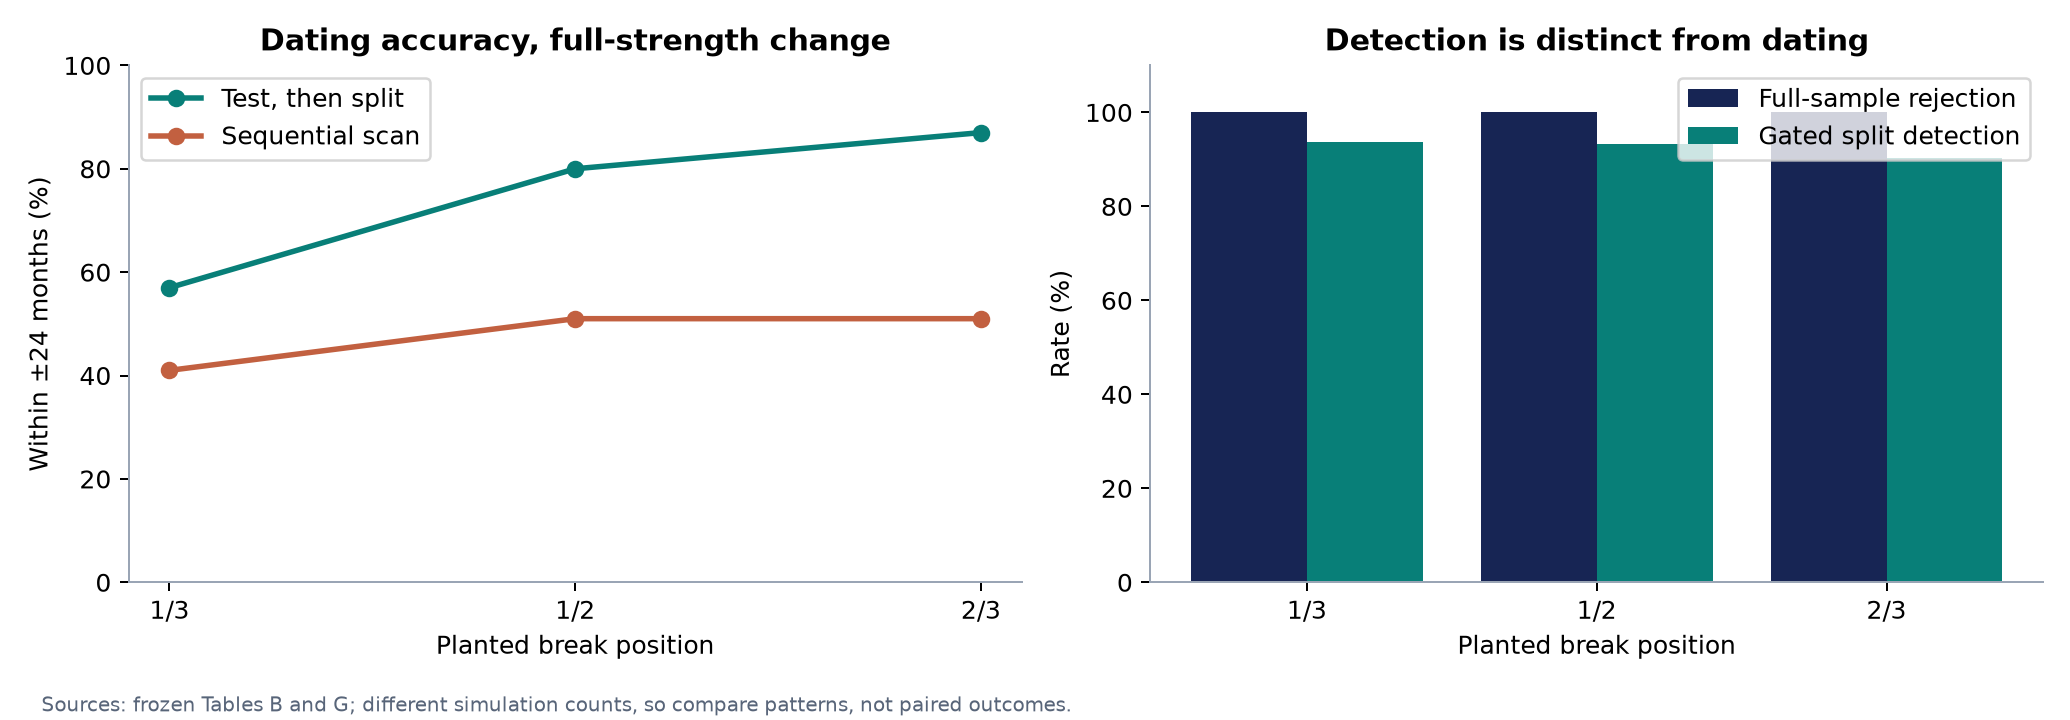
\includegraphics[width=\linewidth]{../figures/06_dating.png}
\caption{Detection and dating are distinct tasks. The left panel shows dates within 24 months of a planted break; the right compares full-sample rejection with gated-split detection. Scan and gated-split figures come from different Monte Carlo cells and are not paired outcomes.}\label{fig.dating}
\end{figure}

As \emph{our addition}, the second procedure separates detection from dating. (a) Run SW's full-sample test at $d$ and level $\alpha$. (b) If it rejects, for every candidate month $k$ (excluding 10\% of the sample at each end, on a six-month grid refined monthly) fit $d$ principal components separately to months before and after $k$, and take as the break the $k$ that minimizes the sum of the two residual sums of squares. Step (b) is the least-squares break estimator used for regressions \citep{Bai1997} and, in a related form, for factor models \citep{BKW2017}. Because the decision is the test's, the procedure's size is the test's size; the date requires no further test.

\begin{table}[htbp]
\centering
\begin{threeparttable}
\caption{Test, then split, on the benchmark (\%, final seeds, 500 panels)}\label{tab.split}
\begin{tabular}{lccccc}
\toprule
 & & \multicolumn{2}{c}{Strength 1} & \multicolumn{2}{c}{Strength 0.5}\\
\cmidrule(lr){3-4}\cmidrule(lr){5-6}
Level & Size & Power & Within 24 mo. & Power & Within 24 mo.\\
\midrule
5\% & 3.8 & 94/93/90 & 57/80/87 & 83/82/70 & 21/39/48\\
1\% & 1.2 & 94/93/90 & 57/80/87 & 70/73/58 & 19/35/40\\
\bottomrule
\end{tabular}
\begin{tablenotes}\small
\item Notes: entries for $\tau=160/240/320$. Power counts a break dated at or after $\tau-12$; the 6--10\% of rejecting panels dated earlier count as misses, which is why power is below the full-sample test's.
\end{tablenotes}
\end{threeparttable}
\end{table}

Table~\ref{tab.split} reports the final-seed results. The size is that of the test, 3.8\% at 5\%. For a change in mid- or late sample with strength 1 the median dating error is zero and 80--87\% of dates fall within 24 months, against about 50\% for the scan. For an early change, or a weak one, the least-squares date is pulled toward the middle of the sample and only 20--57\% fall within 24 months. The procedure dates a single change; a recursive version that splits again on each side reports 1.3--1.6 spurious extra breaks per panel and is not recommended. Two other estimation-based procedures were rejected on the same benchmark: a sup-type test built on the split statistic with its own bootstrap over-rejected at 5\% and 10\% (9\% and 15.5\%), and rolling windows dated by the window midpoint placed most dates before the change.

\subsection{Interpretation}

With these caveats, the dates are best read as episodes rather than months. Pooling the $d=4$ breaks found under three per-window bandwidth rules (the rule of thumb, and $0.5\times$ and $1.5\times$ it) in both panels, they cluster in five episodes: 1981--84 (JKV 1981-08, 1983-04, 1984-12; the peak of the federal funds rate in mid-1981 and the end of monetary targeting in late 1982); 1991--94 (Treasury 1991-09, 1992-06, 1993-06; JKV 1993-09, 1994-05; rate cuts after the 1990--91 recession, then the surprise tightening from February 1994); 2004--06 (Treasury 2004-03; JKV 2004-07, 2004-12, 2006-10; the tightening from 1\% to 5.25\% with little response of long yields); 2008 (Treasury 2008-09 under $0.5\times$ and $1.5\times$; the policy rate reaching zero); and 2019--21 (Treasury 2019-11, 2021-02, 2021-06; rate cuts, the pandemic, and the return of inflation). Many of these dates lie near turns in Federal Reserve policy, but the sample contains many such turns and we do not test the association formally. Given the delays in Table~\ref{tab.scansim}, each change probably began before the date at which the scan records it, and given the weak detection at $d=4$, the absence of a break in a period is not evidence of stability.

\section{A test robust to serially correlated errors}\label{sec.robust}

Sections~\ref{sec.ar} and \ref{sec.discussion} identify serial correlation as the main threat to the empirical rejections. This section, written after the earlier analysis, diagnoses the failure more closely and proposes a version of the test that keeps SW's null hypothesis and their local-versus-global comparison but remains valid with persistent errors. All results here are Monte Carlo or exploratory empirical evidence; we have no asymptotic theory for the new procedure yet.

\subsection{Why the original test fails}\label{sec.robust.why}

\paragraph{The failure is the method's, not the data's.} We first checked that our implementation is SW's test: on the same input matrices, the two statistics computed by the authors' MATLAB routine (run in Octave) agree with our port to twelve significant digits. A by-product of this check is that the bias and variance estimators $\hat B_{NT}$ and $\hat V_{1NT}$ multiply local factors estimated at different dates, so they depend on the arbitrary sign (and rotation) of the local eigenvectors; on one JKV matrix $\hat J_{NT}$ is 60.9 with raw eigenvector signs and 71.3 with a first-row-positive convention. We recommend aligning local loadings to the global ones (Procrustes) and fix the first-row convention throughout. We then added AR errors to SW's own DGP~1 ($N=T=100$, two factors). Figure~\ref{fig.swdgp} shows that SW's test, which has size 2\% with independent errors, rejects 88\% of null panels with AR(0.3) errors and 100\% with AR(0.6). The same holds for the statistics in the authors' code. Over-rejection under persistence is therefore a property of the procedure, not of yield data or of our code.

\begin{figure}[htbp]
\centering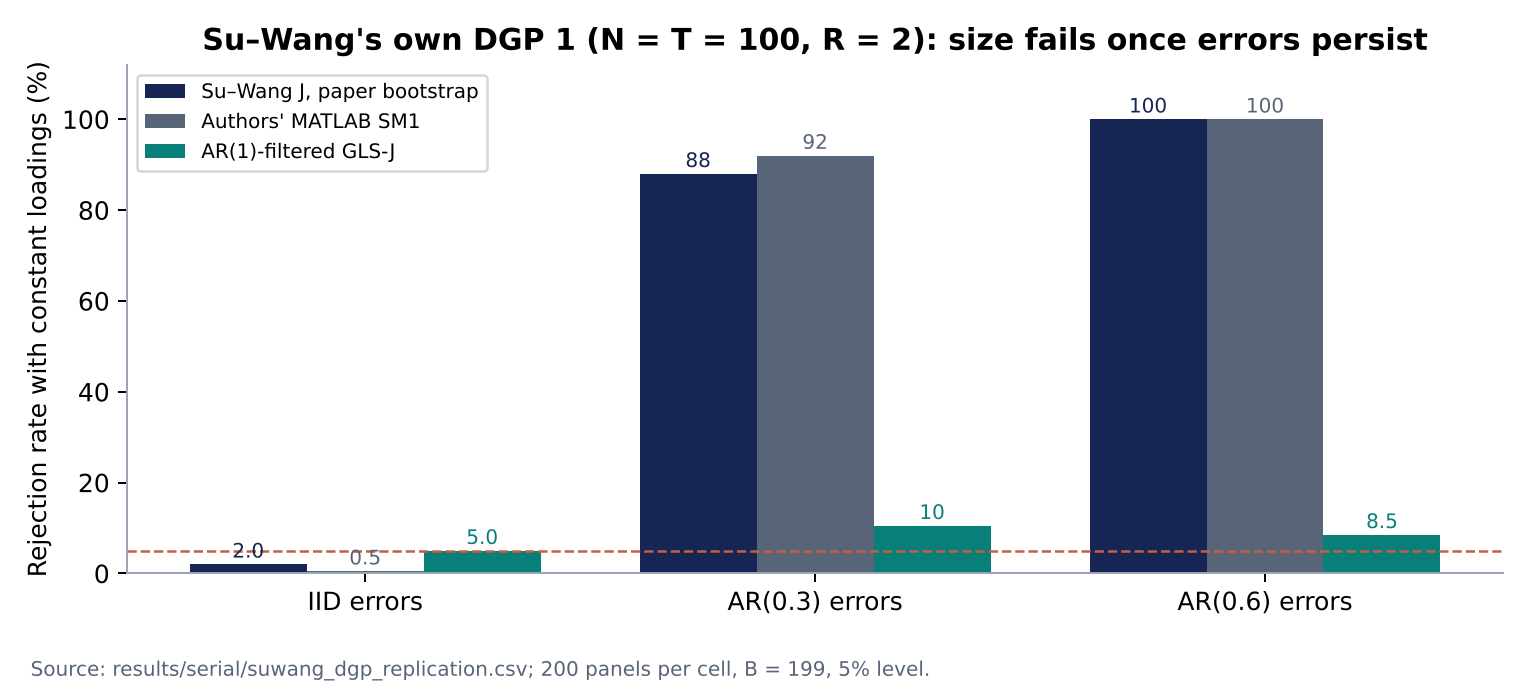
\includegraphics[width=0.85\linewidth]{../figures/08_suwang_dgp_serial.png}
\caption{SW's DGP~1 with AR errors: rejection frequencies under constant loadings (200 panels, $B=199$, 5\% level). The AR(1)-filtered GLS statistic of Section~\ref{sec.robust.method} is shown for comparison; at $T=100$ its size is 8--10\%.}\label{fig.swdgp}
\end{figure}

\paragraph{Narrowing the bandwidth does not help.} When residuals of a factor model with a fixed number of factors remain serially correlated, a natural response is to narrow the bandwidth, so that the local fit follows the data more closely. Figure~\ref{fig.bwpersist} (left) confirms that narrower bandwidths reduce the lag-one autocorrelation of the local residuals in both panels (JKV: from 0.63 for constant loadings to 0.22 at $h=0.25h_0$), but never remove it. The right panel shows the cost: in calibrated simulations with AR(0.3) errors and constant loadings, SW's test rejects 62.5\% of panels at $2h_0$ and 98.5\% at $0.5h_0$ (JKV). A narrow kernel lets the local loadings absorb persistent noise, which the statistic then reads as time variation. Selecting $h$ by blocked cross-validation inside an AR(1) bootstrap restores size (1--4\%) but leaves power at 12--13\% against a half-strength change.

\begin{figure}[htbp]
\centering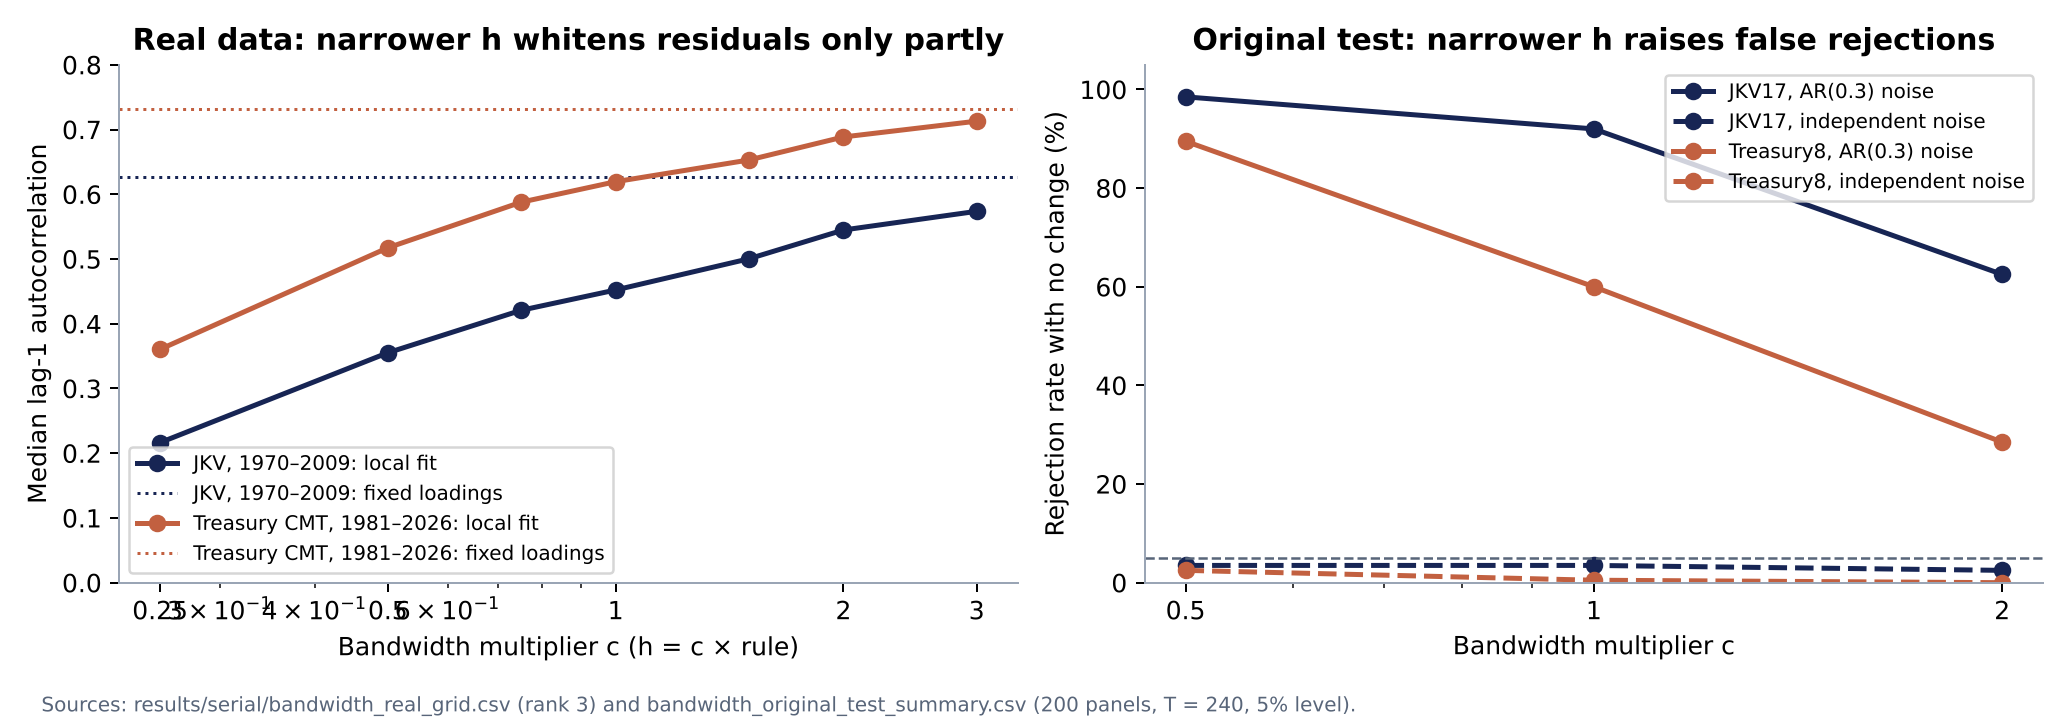
\includegraphics[width=\linewidth]{../figures/07_bandwidth_persistence.png}
\caption{Left: median lag-one autocorrelation of residuals in the real panels, rank 3, as a function of the bandwidth multiplier $c$ ($h=c h_0$); dotted lines are the constant-loading fits. Right: rejection rates of SW's test under constant loadings in calibrated simulations ($T=240$, 200 panels).}\label{fig.bwpersist}
\end{figure}

\paragraph{AR-aware bootstraps trade power for size.} Section~\ref{sec.ar} showed that an AR(1) bootstrap for SW's statistic either controls size and loses power, or the reverse. In the fixed-rank loading-shift design used below, the AR(1) bootstrap based on constant-loading residuals has size 1.0--4.5\% but power of only 7.5\% (JKV) and 23\% (Treasury) against a half-strength loading change with AR(0.6) errors (Table~\ref{tab.robust.sp}). A dependent wild bootstrap \citep{Shao2010} applied to SW's statistic does not control size (12--50\% under AR(0.6)), because $\hat J_{NT}$ is standardized as if the errors were martingale differences.

\subsection{The sieve-AR GLS-J test}\label{sec.robust.method}

The idea is to make the errors unpredictable before comparing local and global loadings, and to put the persistence back in the bootstrap. Let $\hat F_t$ be the first $d$ principal components of the standardized panel and $\hat e_{it}$ the residuals of the constant-loading fit.
\begin{enumerate}
\item \emph{Filter.} Choose one autoregressive order $\hat p\le 6$ for all maturities by minimizing the pooled criterion $\sum_i\log\hat\sigma^2_{u,i}(p)+2Np/T_p$ (AIC), fit $\hat e_{it}=\sum_{j=1}^{\hat p}\phi_{ij}\hat e_{i,t-j}+u_{it}$ maturity by maturity, and quasi-difference yields and factors, $\tilde x_{it}=x_{it}-\sum_j\hat\phi_{ij}x_{i,t-j}$ and $\tilde z_{it}=\hat F_t-\sum_j\hat\phi_{ij}\hat F_{t-j}$, as in the GLS estimator of \citet{BreitungTenhofen2011}.
\item \emph{Compare.} Estimate full-sample loadings $\hat\lambda_i$ by least squares of $\tilde x_{it}$ on $\tilde z_{it}$, and local loadings $\hat\lambda_i(t)$ by kernel-weighted least squares with SW's boundary kernel and bandwidth $h=2h_0$, fixed in advance. The statistic is the regression form of SW's comparison \citep{SuWang2020},
\[
\hat M_{GLS}=\frac{1}{NT}\sum_{i=1}^N\sum_{t}\frac{\big[(\hat\lambda_i(t)-\hat\lambda_i)'\tilde z_{it}\big]^2}{\hat\sigma^2_{u,i}},
\]
with $\hat\sigma^2_{u,i}$ the variance of the filtered residual of maturity $i$.
\item \emph{Calibrate.} Draw $u^*_{it}=\hat u_{it}\eta_t$ with one Rademacher sign $\eta_t$ per month shared by all maturities (which keeps the cross-maturity correlation), rebuild $e^*_{it}$ through the fitted AR($\hat p$) recursion, form $x^*_{it}$ as the fitted common component plus $e^*_{it}$, and recompute $\hat M_{GLS}$ after re-estimating factors, AR coefficients and loadings, with $\hat p$ held fixed. The $p$-value is the add-one share of $B$ draws at or above the observed statistic. This is a sieve bootstrap in the sense of \citet{Kreiss1992} and \citet{Buhlmann1997}.
\end{enumerate}
The null hypothesis, the kernel and the local-versus-global comparison are SW's; what is new is that the noise is whitened first, the AR order is chosen from the data, and the bootstrap carries the dynamics. The statistic is not centred or studentized and relies on the bootstrap for its null distribution. The released implementation (\texttt{code/serial\_robust.py}) reproduces the exploratory code on which the simulations were run, panel by panel: on 40 test panels the $p$-values, decisions, numbers of bootstrap draws and AR orders are identical.

\subsection{Size and power}\label{sec.robust.mc}

The simulations use $T=240$ months, Nelson--Siegel calibrations to JKV (17 maturities, 1970--2009) and to the eight-maturity Treasury curve (1990--2009), 250 panels per cell and $B=199$. Unlike the benchmark of Section~\ref{sec.bench}, the main alternative keeps three factors and shifts the loadings at mid-sample: from $T/2$ the third factor also loads on the fourth Svensson shape, scaled to a share (``strength'') of the calibrated fourth-factor scale. Table~\ref{tab.robust.sp} compares the new test with SW's test and the AR(1) bootstrap on the same design.

\begin{table}[htbp]
\centering
\begin{threeparttable}
\small
\caption{Size / power (\%) at 5\%: SW's test, AR(1) bootstrap and sieve-AR GLS-J}\label{tab.robust.sp}
\begin{tabular}{lcccccc}
\toprule
& \multicolumn{2}{c}{SW's test} & \multicolumn{2}{c}{+ AR(1) bootstrap} & \multicolumn{2}{c}{Sieve-AR GLS-J}\\
\cmidrule(lr){2-3}\cmidrule(lr){4-5}\cmidrule(lr){6-7}
Errors & JKV & Treasury & JKV & Treasury & JKV & Treasury\\
\midrule
Independent & 3.5 / 44.0 & 3.5 / 72.5 & 3.5 / 39.0 & 3.5 / 68.0 & 2.4 / 49.6 & 1.2 / 76.8\\
AR(0.3) & 95.0 / 99.5 & 62.5 / 97.0 & 3.0 / 18.0 & 4.5 / 35.0 & 1.6 / 26.4 & 1.2 / 55.2\\
AR(0.6) & 100 / 100 & 100 / 100 & 1.0 / 7.5 & 1.5 / 23.0 & 2.4 / 20.8 & 2.0 / 44.4\\
\bottomrule
\end{tabular}
\begin{tablenotes}\small
\item Notes: size under constant loadings; power against a half-strength loading shift at $T/2$. SW's test and the AR(1) bootstrap: 200 panels; sieve-AR GLS-J: 250 panels. When the size is far above 5\%, the accompanying power is mostly false rejection. Sources: \texttt{results/serial/ar\_bootstrap\_study\_summary.csv} and \texttt{simulation\_all\_runs\_summary.csv}.
\end{tablenotes}
\end{threeparttable}
\end{table}

Figure~\ref{fig.robust.size} reports the size of the new test over sixteen error designs: homogeneous AR(1) with coefficients from 0 to 0.9, AR coefficients rising from 0.2 to 0.7 across maturities, AR(2), ARMA(1,1), a persistent AR(0.95) component plus measurement noise, constant cross-maturity correlation, a switch to cross-maturity correlation at mid-sample, a proportional 50\% volatility increase at every maturity, and true rank four tested with $d=4$. In 27 of the 32 cells the size lies between 0.8\% and 7.6\%. The exceptions are JKV with rank four and independent errors (10.4\%), where the fourth factor is weak, and the case discussed in Section~\ref{sec.robust.ident}.

\begin{figure}[htbp]
\centering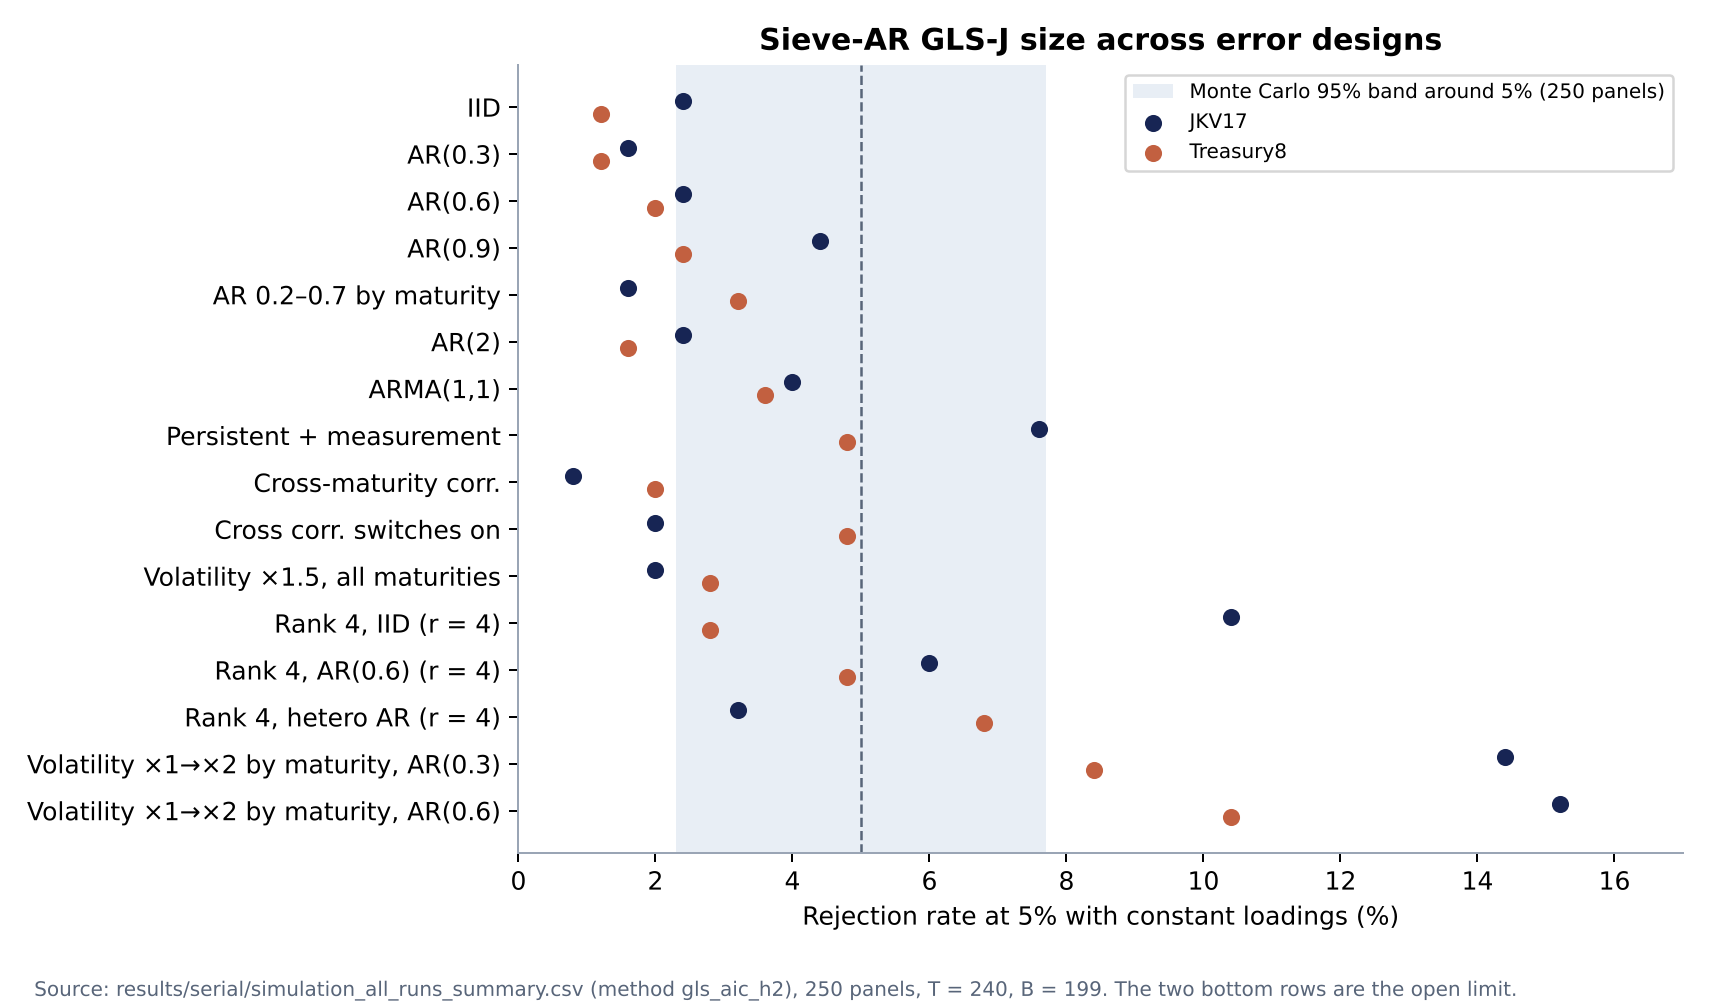
\includegraphics[width=0.8\linewidth]{../figures/09_sieve_gls_size.png}
\caption{Size of sieve-AR GLS-J at 5\% under constant loadings, 16 error designs, two calibrations (250 panels each). The shaded band is the Monte Carlo 95\% interval around 5\%.}\label{fig.robust.size}
\end{figure}

\begin{figure}[htbp]
\centering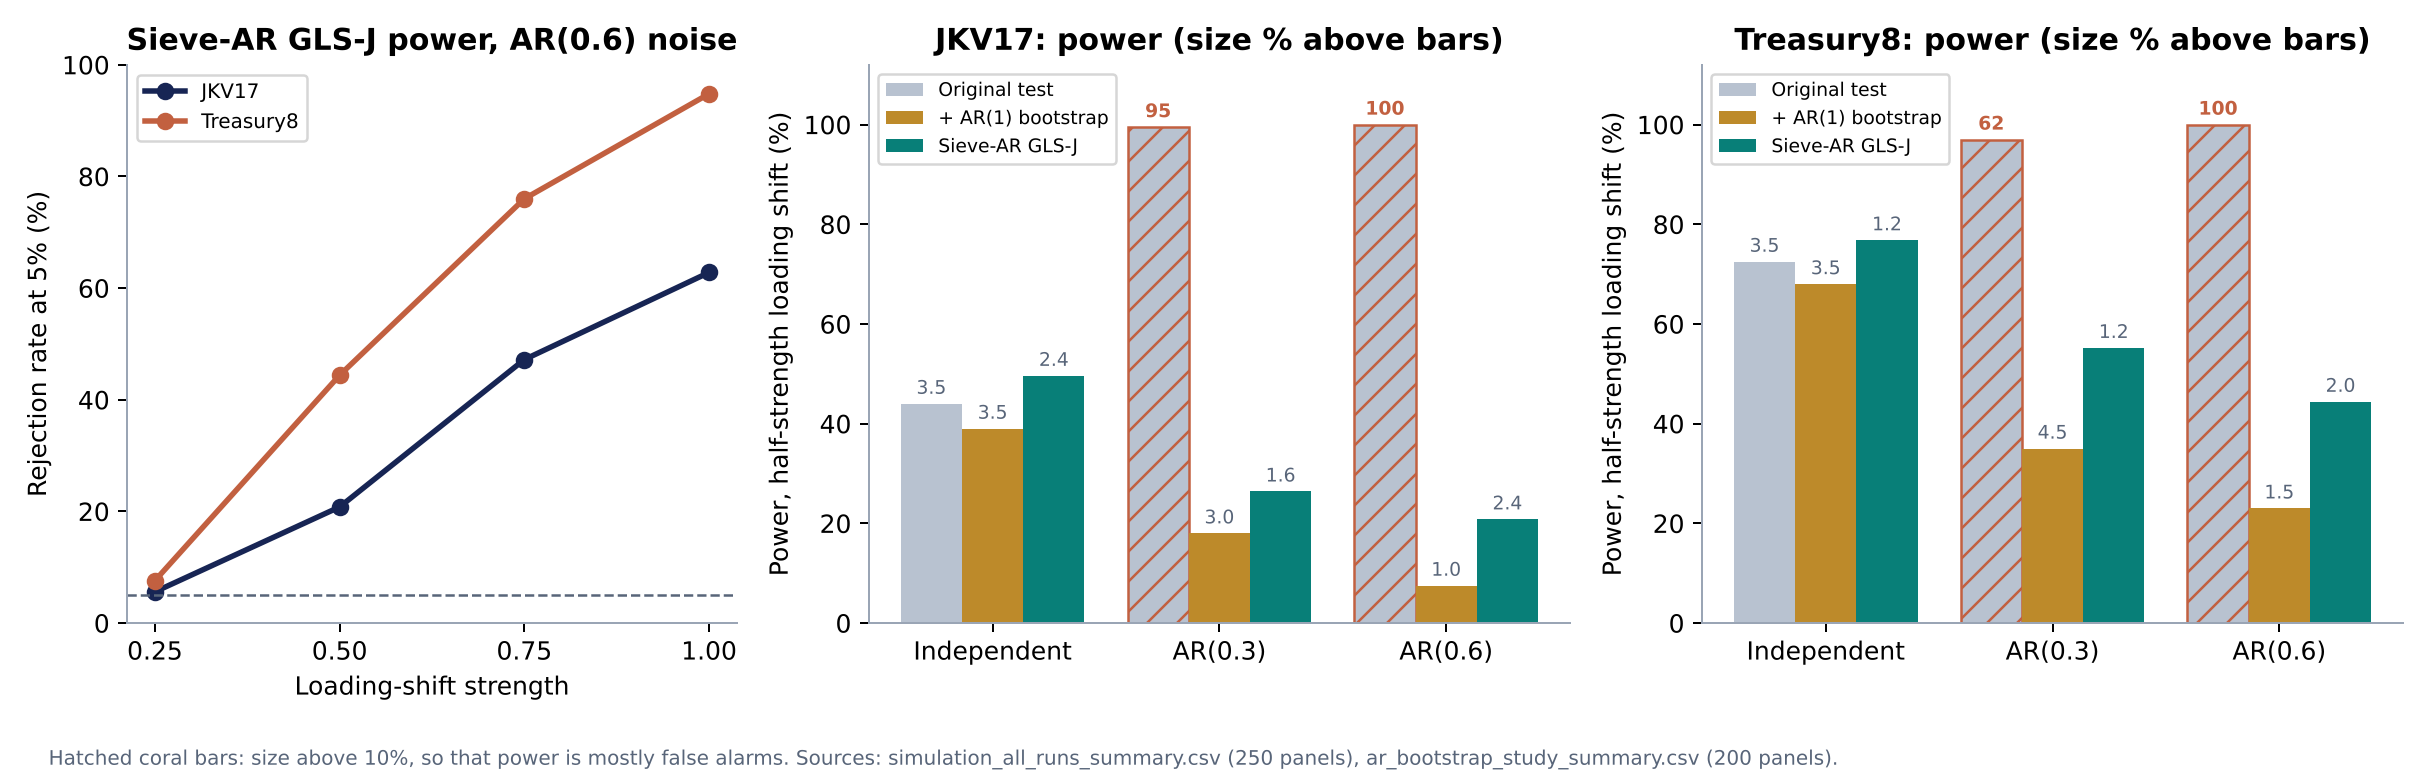
\includegraphics[width=\linewidth]{../figures/10_sieve_gls_power.png}
\caption{Left: power of sieve-AR GLS-J against loading shifts of increasing strength with AR(0.6) errors. Middle and right: power against a half-strength shift, by method and error design, with the size printed above each bar; hatched bars have size above 10\%.}\label{fig.robust.power}
\end{figure}

Power increases with the size of the change (Figure~\ref{fig.robust.power}): with AR(0.6) errors it is 5.6, 20.8, 47.2 and 62.8\% (JKV) and 7.6, 44.4, 76.0 and 94.8\% (Treasury) at strengths 0.25, 0.5, 0.75 and 1. It is 63.2/90.8\% for a full-strength shift with ARMA(1,1) errors and 74.0/72.0\% when a fourth factor appears at mid-sample with AR(0.6) errors. Table~\ref{tab.robust.abl} shows why the order is chosen by AIC and the bandwidth doubled: a fixed AR(1) filter fails when the errors are ARMA(1,1) or contain measurement noise, BIC chooses orders that are too short, and $h=2h_0$ raises power with no cost in size. Bias-correcting the AR coefficients, iterating the factor estimates, local variance weights and applying SW's $\hat J_{NT}$ to the quasi-differenced data did not improve on the baseline.

\begin{table}[htbp]
\centering
\begin{threeparttable}
\small
\caption{Design choices: rejection rates (\%, JKV / Treasury) on the same panels}\label{tab.robust.abl}
\begin{tabular}{lccc}
\toprule
Variant & ARMA(1,1) size & Measurement-noise size & Power, AR(0.6), 0.5\\
\midrule
Fixed AR(1) filter, $h_0$ & 73.6 / 47.6 & 100 / 98.0 & 19.2 / 34.0\\
Sieve, BIC order, $h_0$ & 13.2 / 16.8 & 55.6 / 34.4 & 19.2 / 33.6\\
Fixed AR(1) filter, $2h_0$ & 40.0 / 23.2 & 99.2 / 83.2 & 20.8 / 44.4\\
Sieve, AIC order, $2h_0$ (adopted) & 4.0 / 3.6 & 7.6 / 4.8 & 20.8 / 44.4\\
\bottomrule
\end{tabular}
\begin{tablenotes}\small
\item Notes: 250 panels, $T=240$, $B=199$. Source: \texttt{results/serial/simulation\_all\_runs\_summary.csv} (methods \texttt{gls\_M\_wild}, \texttt{gls\_sieve}, \texttt{gls\_h2}, \texttt{gls\_aic\_h2}).
\end{tablenotes}
\end{threeparttable}
\end{table}

\subsection{An identification limit}\label{sec.robust.ident}

Writing $y_t=\Lambda_3f_t+\lambda_4g_t+e_t$ as $y_t=\Lambda_3f_t+e^*_t$ with $e^*_t=\lambda_4g_t+e_t$ shows that, if the error covariance may change arbitrarily, a new common factor and a new common component of the errors are observationally equivalent. Any test must therefore restrict how the errors may change. The new test is robust to two such changes---a proportional change in error volatility at all maturities and a change in cross-maturity correlation (size 2.0--4.8\%)---whereas a conditional Nelson--Siegel shape test that we also considered rejects 93--99\% of panels when only the error volatility rises by half. It is not robust to a volatility change that differs across maturities: when, after mid-sample, the error standard deviation is multiplied by factors rising linearly from 1 at the shortest to 2 at the longest maturity, its size is 14.4--15.2\% (JKV) and 8.4--10.4\% (Treasury). Such a change rotates the estimated factor space, which the statistic reads as a loading change. A $T$-dependent maximum AR order does not change this, and weighting the principal components separately in the two halves makes it worse (21--84\%). We therefore state stable \emph{relative} error volatility within a test window as an assumption. In the 1990--2009 data the ratio of second-half to first-half residual standard deviations is 1.03--1.92 (JKV) and 1.05--1.48 (Treasury), so this assumption is not innocuous.

\subsection{Exploratory empirical results}\label{sec.robust.emp}

Table~\ref{tab.robust.emp} and Figure~\ref{fig.robust.emp} apply the new test to the real panels with $B=999$. These runs were not pre-registered; the specification (samples, order of ranks, maximum AR order, bandwidth) will be fixed before a confirmatory run. Over 1990--2009, constant three-factor loadings are rejected in both panels ($p=0.026$ and 0.005), whereas constant four-factor loadings are not ($p=0.196$ and 0.350). Part of the apparent three-factor loading change may therefore be an omitted fourth factor, in line with the hidden factor of \citet{Duffee2011}. In 1970--1989 the AIC order reaches its upper bound of six, and allowing up to twelve lags moves the three-factor $p$-value from 0.007 to 0.050. The 2010--2026 Treasury sample rejects at both ranks, but it contains the zero-lower-bound years, in which short-maturity volatility nearly vanishes---the case of Section~\ref{sec.robust.ident}---so we do not interpret it.

\begin{table}[htbp]
\centering
\begin{threeparttable}
\small
\caption{Sieve-AR GLS-J on the real panels (bootstrap $p$-values, $B=999$)}\label{tab.robust.emp}
\begin{tabular}{lccccc}
\toprule
Sample & $T$ & $d=3$ & $d=4$ & $d=3$, $p_{\max}=12$ & $d=4$, $p_{\max}=12$\\
\midrule
JKV 1970--1989 & 240 & 0.007 & 0.001 & 0.050 & 0.049\\
JKV 1990--2009 & 240 & 0.026 & 0.196 & 0.022 & 0.195\\
JKV 1970--2009 & 480 & 0.001 & 0.001 & 0.001 & 0.001\\
Treasury 1990--2009 & 240 & 0.005 & 0.350 & 0.005 & 0.350\\
Treasury 1990--2026 & 440 & 0.003 & 0.108 & 0.002 & 0.108\\
Treasury 2010--2026 & 200 & 0.001 & 0.001 & 0.001 & 0.001\\
\bottomrule
\end{tabular}
\begin{tablenotes}\small
\item Notes: AIC order with maximum 6 unless stated; $h=2h_0$; yields in levels. Treasury: eight maturities from the H.15 file in the repository, through August 2026. The exploratory run that preceded it also used a partial September 2026 observation and gave $p=0.005/0.095$ (1990--2026). JKV results are from the licensed panel, which is not redistributed. Sources: \texttt{results/serial/empirical\_*.csv}.
\end{tablenotes}
\end{threeparttable}
\end{table}

\begin{figure}[htbp]
\centering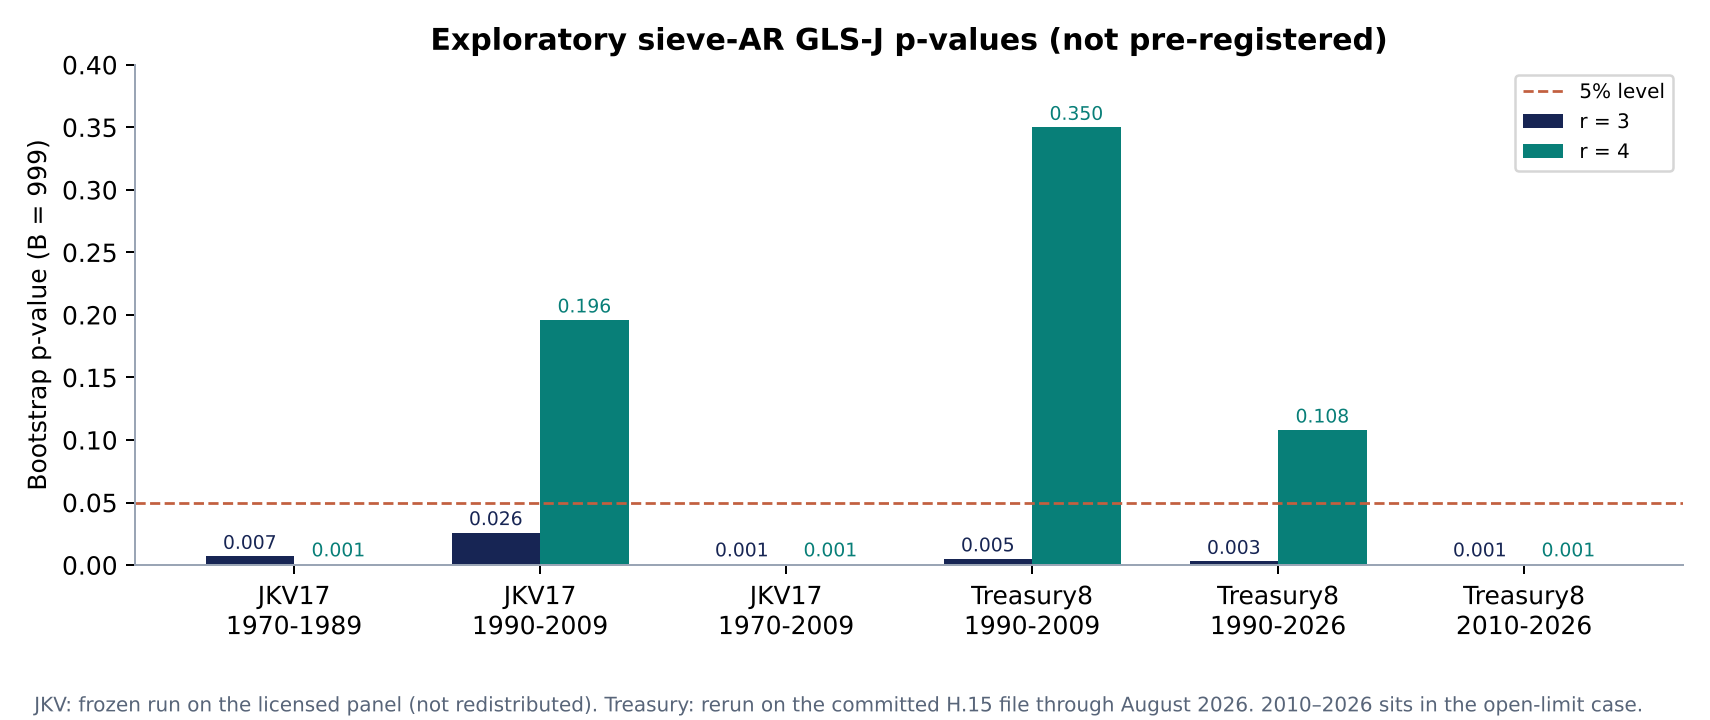
\includegraphics[width=0.85\linewidth]{../figures/11_empirical_pvalues.png}
\caption{Exploratory sieve-AR GLS-J $p$-values ($B=999$); the dashed line marks 5\%.}\label{fig.robust.emp}
\end{figure}

\section{Discussion}\label{sec.discussion}

\paragraph{What the rejections establish.} Under SW's assumptions---errors that are martingale differences over time, and the rank-padding argument of Proposition~\ref{prop.rank}, which our simulations support---the Treasury results reject every constant-loading model with up to five factors and the Fama--Bliss results reject constant three-factor models. In SW's normalization, a change in the variance of a factor is a change in the loadings, so a rejection does not distinguish between ``maturities' sensitivities changed'' and ``a factor became more or less important''. The last row of Table~\ref{tab.fakesize} shows that the test detects the latter.

\paragraph{Serial correlation.} The main limitation is serial correlation. SW's asymptotic theory, not only the bootstrap, requires serially uncorrelated errors, while the residuals of the constant-loading fits have lag-one autocorrelations of 0.5--0.7. Persistent errors make the local fit track the noise more closely than independent errors would, which can raise $\hat J_{NT}$ relative to its bootstrap distribution. The empirical rejections must therefore be read conditional on this assumption. An earlier draft argued that the strength of the rejections---$\hat J_{NT}$ exceeds the 99\% critical value by factors of 4 to 21 at $d=3$ (Tables~\ref{tab.full} and \ref{tab.sub})---made it unlikely that serial correlation alone accounts for them. The simulations of Section~\ref{sec.ar} do not support that argument: with AR(1) errors at $\rho=0.5$ the statistic in a null model is about four times the 5\% critical value (the 99\% value is somewhat larger), so ratios of the same order as the lower end of the empirical range can arise from serial correlation alone. The empirical rejections should be revisited once a bootstrap that reproduces serial correlation is settled; Section~\ref{sec.robust} takes a first step, and its exploratory results confirm the three-factor rejections over 1990--2009 but not the four-factor ones. One fact that the simulations do not yet explain is that the Fama--Bliss panel does not reject at $d=4$ or $d=5$ ($p=0.34$ and 0.26); the residuals of four- and five-factor fits may be less persistent than those of three-factor fits, which we have not checked.

\paragraph{The zero lower bound.} One economic mechanism for loading changes is visible in the sub-samples. When the policy rate is pinned at zero, short-maturity yields stop responding to the factors that move the rest of the curve, which in a factor model is a change in their loadings. Consistent with this, the Treasury panel does not reject at $d=5$ over 1990--2009 or over 2010--2026 separately, but rejects over 1990--2026 and 1981--2026, the samples that span the onset of the zero lower bound (Table~\ref{tab.sub}). This reading is suggestive rather than tested.

\section{Conclusion}\label{sec.conclusion}

Applying the test of \citet{SuWang2017} to two U.S.\ Treasury panels, we find evidence that factor models with time-invariant loadings are not adequate for the yield curve. The official Treasury curve rejects constant loadings with three, four and five factors; the Fama--Bliss curve rejects with three factors over 1970--2009 and with four in every sample starting between 1977 and 1986. The exception is consistent with a loss of power caused by the 1970s rather than support for constant loadings. With serially independent errors the test is close to correctly sized and powerful at our sample sizes, but with errors as persistent as the empirical residuals its bootstrap over-rejects badly, so the rejections are not yet conclusive. Dating the changes is a secondary question beyond SW's test; in simulations, testing once and estimating the date by least squares is more accurate than a sequential scan, which dates changes about 20 months late. On the data, the scan suggests that the loadings shift around a few episodes of monetary-policy change, but these dates are approximate and conditional on the serial-correlation issue.

Two limitations deserve emphasis. First, the test's theory and bootstrap assume errors uncorrelated over time, the empirical residuals are autocorrelated, and in simulations this alone produces rejections; a bootstrap that reproduces serial correlation is needed before the rejections can be read as evidence of changing loadings. The sieve-AR GLS-J test of Section~\ref{sec.robust} keeps its size under a wide range of persistent error designs; on exploratory runs it rejects constant three-factor loadings but not constant four-factor loadings over 1990--2009. It still over-rejects when error volatility changes unevenly across maturities, it has no asymptotic theory yet, and its empirical specification must be fixed before a confirmatory run. Second, the break dates depend on the bandwidth rule and the search settings, and wide bandwidths in short windows lie outside the theory of the test. For applied work the implication is that yield-curve models should allow the loadings to change over time, or at least be estimated on samples within which they are stable.

\section*{Data and code availability}

The Fama--Bliss panel is from the \emph{Journal of Applied Econometrics} data archive entry of \citet{JKV2014}; the underlying data are from the CRSP Monthly Treasury files, on which CRSP retains copyright. Treasury CMT yields are from the Federal Reserve H.15 release and treasury.gov. The Python implementation, simulation code, random seeds and summary results accompany this working draft in the public repository; the serial-correlation-robust test is in \texttt{code/serial\_robust.py}, its summaries in \texttt{results/serial/}, and the full sequence of analyses in \texttt{notebook/research\_notebook.ipynb}. CRSP source yields are not redistributed.

\appendix

\section{The bootstrap in the released code}\label{app.bootstrap}

The bootstrap of SW, Section 4.6, draws errors $e^*_t=\tilde\Sigma^{1/2}\varsigma_t$ that reproduce the cross-sectional covariance of the residuals. In the MATLAB code released with the paper, as we obtained it , the draws are produced by a routine (\texttt{MultiNormal.m}) that starts from the diagonal square root $\mathrm{diag}(\tilde\sigma_{ii}^{1/2})$ and uses the Cholesky factor of the covariance only if the Cholesky decomposition fails. Because the caller adds a small ridge, it does not fail, so the bootstrap errors generated by the code as released are independent across units. The same routine generates the errors of SW's DGP 3, so in the code as released the ``cross-correlated'' design of SW's Table 3 generates independent errors.

Run the way the code runs, our implementation reproduces SW's Table 3: in a 300-replication run with $B=99$, 22 of 24 size cells lie within two Monte Carlo standard errors of the published values, and the power in Table 4 matches (e.g.\ DGP 4, $b=1$, $N=T=100$: 100\% against 99.8\%). At $N=T=100$ under DGP 1 the size at 5\% is 1.2\% with the printed covariance bootstrap, 3.9\% with diagonal errors, 7.0\% with diagonal errors and re-standardized draws, 7.5\% with the code as it runs, and 6.4\% in SW.

The distinction matters for yield curves, whose residuals are strongly cross-correlated. With truly cross-correlated errors ($0.5^{|i-j|}$), the code's bootstrap rejects 17--21\% of the time at a 5\% level for $N,T\in\{100,200\}$; at our sample sizes it rejects 12--82\%. The printed bootstrap keeps size at 5--7\%. We therefore use the printed version throughout.

\section{Boundary kernel for wide bandwidths}\label{app.kernel}

The boundary kernel (\ref{eq.boundary}) renormalizes $K$ by its mass inside the sample on one side only. In SW's simulations ($T\in\{100,200\}$) $Th<T/2$, the two boundary regions never overlap, and the formula is complete. When the full-sample bandwidth is reused in a short scan window, $h$ can exceed $1/2$ (for JKV, $h=1.19$, 0.60 and 0.30 in windows of 60, 120 and 240 months), and dates near the middle of the window fall in both boundary regions. Applying (\ref{eq.boundary}) as written---as in the released code---lets the right-hand correction overwrite the left, and the weights on a date then sum to between 0.50 and 0.97.

We use the cut-and-normalize rule of \citet{HongLi2005}, \citet{LiRacine2007} and \citet{Jones1993}, of which (\ref{eq.boundary}) is the one-sided case: for every $r$,
\[
  k^*_{h,tr}=h^{-1}K\!\left(\frac{t-r}{Th}\right)\Big/\int_{\max\{-1,\,-r/(Th)\}}^{\min\{1,\,(1-r/T)/h\}}K(u)\,du.
\]
Where the boundary regions do not overlap this coincides with (\ref{eq.boundary}) exactly, and all per-window results are reproduced to the last digit. Figure~\ref{fig.kernel} shows the weights in a 60-month window with $Th=71.4$. Only the kernel weights are modified; the bias and variance terms in (\ref{eq.J}) keep SW's form, so $\hat J_{NT}$ values from windows of different lengths are not directly comparable and we compare only bootstrap $p$-values.

\begin{figure}[htbp]
\centering
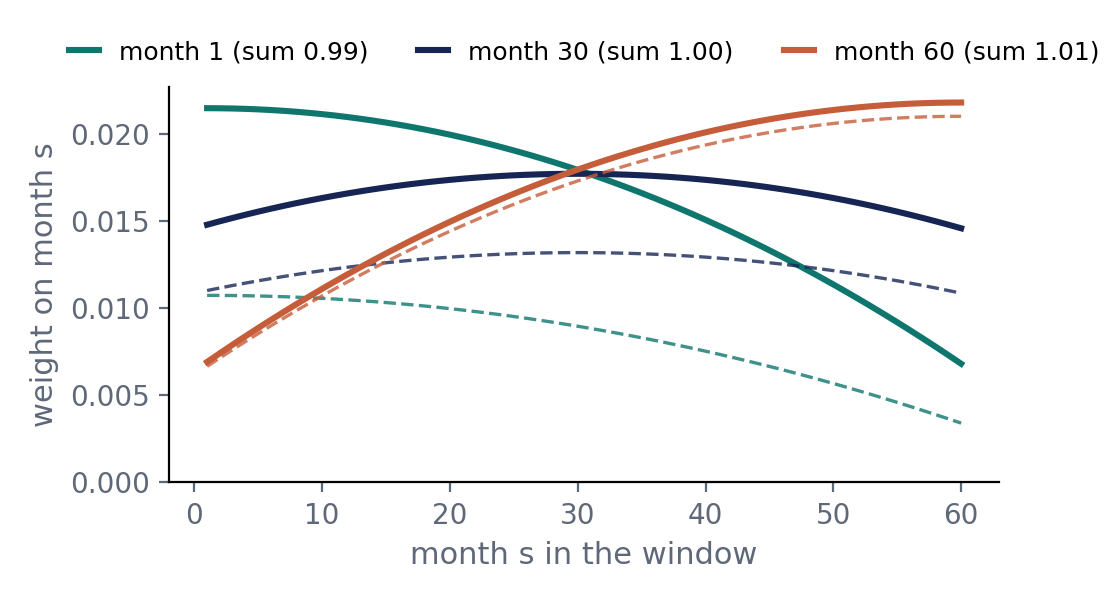
\includegraphics[width=0.75\linewidth]{figures/kernel_60m.png}
\caption{Kernel weights in a 60-month window with $Th=71.4$ months, for target months 1, 30 and 60. Solid: two-sided cut-and-normalize rule (weights sum to one). Dashed: the one-sided formula applied with overlapping boundary regions.}\label{fig.kernel}
\end{figure}

\section{Additional dating experiments}\label{app.dating}

\paragraph{Can the scan be tuned?} As \emph{our addition}, and with a selection rule written before the run, we evaluated 18 scan rules on the same panels: first and restart window $W\in\{36,60,120\}$ months, retreat on or off, and a per-window level $\alpha_w\in\{1\%,0.5\%,0.2\%\}$ (a proof of concept on 100 null panels and 30 break panels per strength at $\tau=240$, with no final-seed check). The window length barely matters, and retreat is rarely triggered and never changes the first date. Lowering $\alpha_w$ brings the size of the procedure from 6--7\% down to 3\%, but makes the dates later: the share within 24 months falls from 63\% to 53\% at strength 1, and is 0--7\% at strength 0.5 under every rule. The selected rule ($W=120$, $\alpha_w=1\%$) has size 5\%, a median delay of 20 months and 63\% of dates within 24 months. Tuning thus controls the scan's size but not its dating, which confirms that the delay comes from the rule rather than its settings.

\subsection*{Other dating statistics: a proof of concept}\label{sec.newstat}

As \emph{our addition}, we compared the least-squares split with three bootstrap-free statistics that target the change more directly: a two-sided window statistic in the spirit of MOSUM, which compares the $d=3$ fit of $h$ months before and after each $t$ ($h=60$ or 96); the change in the fourth eigenvalue (or the ratio of the fourth to the fifth) between the two windows, which targets the appearance of a fourth factor; and the distance between the three-dimensional principal subspaces of the two windows, a direct measure of loading change. Each statistic dates the change at its maximum. To compare them quickly we set the critical value at the 95\% quantile of the maximum on 200 null panels; this uses the known data-generating process and is available only in simulation. Size is measured on 200 other null panels and dating on 100 break panels per cell.

The least-squares split dates best (69, 81 and 81\% within 24 months at strength 1 for $\tau=160$, 240 and 320). Two-sided windows of 96 months are unbiased but less precise (50--66\%), and 60-month windows date late. The eigenvalue and subspace statistics have almost no power (0--24\%): the fourth factor's loading lies 95\% in the span of the first three, so its arrival barely moves the fourth eigenvalue or rotates the leading subspace. With AR(1) noise at $\rho=0.5$ and the same critical values, every statistic that has power also over-rejects (size 100\%), but the least-squares date remains accurate (68\% within 24 months at $\tau=240$). Serial correlation therefore damages the decision whether there is a change, not the estimate of when. This points to combining an autocorrelation-robust test with least-squares dating.

\begin{thebibliography}{99}

\bibitem[Bai(1997)]{Bai1997}
Bai, J. (1997). Estimation of a change point in multiple regression models. \emph{Review of Economics and Statistics}, 79(4), 551--563.

\bibitem[Bai(2003)]{Bai2003}
Bai, J. (2003). Inferential theory for factor models of large dimensions. \emph{Econometrica} 71, 135--171.

\bibitem[Bai and Ng(2002)]{BaiNg2002}
Bai, J. and Ng, S. (2002). Determining the number of factors in approximate factor models. \emph{Econometrica} 70, 191--221.

\bibitem[Baltagi et al.(2017)]{BKW2017}
Baltagi, B. H., Kao, C., and Wang, F. (2017). Identification and estimation of a large factor model with structural instability. \emph{Journal of Econometrics}, 197(1), 87--100.

\bibitem[Bowsher and Meeks(2008)]{BowsherMeeks2008}
Bowsher, C.~G. and Meeks, R. (2008). The dynamics of economic functions: modeling and forecasting the yield curve. \emph{Journal of the American Statistical Association} 103, 1419--1437.

\bibitem[Breitung and Eickmeier(2011)]{BreitungEickmeier2011}
Breitung, J. and Eickmeier, S. (2011). Testing for structural breaks in dynamic factor models. \emph{Journal of Econometrics} 163, 71--84.

\bibitem[Breitung and Tenhofen(2011)]{BreitungTenhofen2011}
Breitung, J. and J.~Tenhofen (2011). GLS estimation of dynamic factor models. \emph{Journal of the American Statistical Association} 106(495), 1150--1166.

\bibitem[B\"uhlmann(1997)]{Buhlmann1997}
B\"uhlmann, P. (1997). Sieve bootstrap for time series. \emph{Bernoulli} 3(2), 123--148.

\bibitem[Chen et al.(2014)]{CDG2014}
Chen, L., Dolado, J.~J. and Gonzalo, J. (2014). Detecting big structural breaks in large factor models. \emph{Journal of Econometrics} 180, 30--48.

\bibitem[Christensen et al.(2011)]{CDR2011}
Christensen, J.~H.~E., Diebold, F.~X. and Rudebusch, G.~D. (2011). The affine arbitrage-free class of Nelson--Siegel term structure models. \emph{Journal of Econometrics} 164, 4--20.

\bibitem[Diebold and Li(2006)]{DieboldLi2006}
Diebold, F.~X. and Li, C. (2006). Forecasting the term structure of government bond yields. \emph{Journal of Econometrics} 130, 337--364.

\bibitem[Duffee(2011)]{Duffee2011}
Duffee, G.~R. (2011). Information in (and not in) the term structure. \emph{Review of Financial Studies} 24(9), 2895--2934.

\bibitem[Fama and Bliss(1987)]{FamaBliss1987}
Fama, E.~F. and Bliss, R.~R. (1987). The information in long-maturity forward rates. \emph{American Economic Review} 77, 680--692.

\bibitem[G\"urkaynak et al.(2007)]{GSW2007}
G\"urkaynak, R.~S., Sack, B. and Wright, J.~H. (2007). The U.S. Treasury yield curve: 1961 to the present. \emph{Journal of Monetary Economics} 54, 2291--2304.

\bibitem[Han and Inoue(2015)]{HanInoue2015}
Han, X. and Inoue, A. (2015). Tests for parameter instability in dynamic factor models. \emph{Econometric Reviews} 34.

\bibitem[Hong and Li(2005)]{HongLi2005}
Hong, Y. and Li, H. (2005). Nonparametric specification testing for continuous-time models with applications to term structure of interest rates. \emph{Review of Financial Studies} 18, 37--84.

\bibitem[Jones(1993)]{Jones1993}
Jones, M.~C. (1993). Simple boundary correction for kernel density estimation. \emph{Statistics and Computing} 3, 135--146.

\bibitem[Jungbacker et al.(2014)]{JKV2014}
Jungbacker, B., Koopman, S.~J. and van der Wel, M. (2014). Smooth dynamic factor analysis with application to the U.S. term structure of interest rates. \emph{Journal of Applied Econometrics} 29, 65--90.

\bibitem[Koopman et al.(2010)]{KMV2010}
Koopman, S.~J., Mallee, M.~I.~P. and van der Wel, M. (2010). Analyzing the term structure of interest rates using the dynamic Nelson--Siegel model with time-varying parameters. \emph{Journal of Business \& Economic Statistics} 28, 329--343.

\bibitem[Kreiss(1992)]{Kreiss1992}
Kreiss, J.-P. (1992). Bootstrap procedures for AR($\infty$)-processes. In K.-H. J\"ockel, G.~Rothe and W.~Sendler (eds.), \emph{Bootstrapping and Related Techniques}, Lecture Notes in Economics and Mathematical Systems 376, 107--113. Berlin: Springer.

\bibitem[Li and Racine(2007)]{LiRacine2007}
Li, Q. and Racine, J.~S. (2007). \emph{Nonparametric Econometrics: Theory and Practice}. Princeton University Press.

\bibitem[Litterman and Scheinkman(1991)]{LittermanScheinkman1991}
Litterman, R. and Scheinkman, J. (1991). Common factors affecting bond returns. \emph{Journal of Fixed Income} 1, 54--61.

\bibitem[Nelson and Siegel(1987)]{NelsonSiegel1987}
Nelson, C.~R. and Siegel, A.~F. (1987). Parsimonious modeling of yield curves. \emph{Journal of Business} 60, 473--489.

\bibitem[Shao(2010)]{Shao2010}
Shao, X. (2010). The dependent wild bootstrap. \emph{Journal of the American Statistical Association} 105(489), 218--235.

\bibitem[Su and Wang(2017)]{SuWang2017}
Su, L. and Wang, X. (2017). On time-varying factor models: estimation and testing. \emph{Journal of Econometrics} 198, 84--101.

\bibitem[Su and Wang(2020)]{SuWang2020}
Su, L. and X.~Wang (2020). Testing for structural changes in factor models via a nonparametric regression. \emph{Econometric Theory} 36(6), 1127--1158.

\bibitem[Svensson(1994)]{Svensson1994}
Svensson, L.~E.~O. (1994). Estimating and interpreting forward interest rates: Sweden 1992--1994. NBER Working Paper 4871.

\bibitem[Yamamoto and Tanaka(2015)]{YamamotoTanaka2015}
Yamamoto, Y. and Tanaka, S. (2015). Testing for factor loading structural change under common breaks. \emph{Journal of Econometrics}.

\end{thebibliography}

\end{document}
